\documentclass[11pt]{article}
% Load Packages
%%%%%%%%%%%%%%%%%=
\usepackage[margin=1in]{geometry}
\geometry{letterpaper}
\addtolength{\oddsidemargin}{-0.3in}
\addtolength{\topmargin}{-0.3in}
\addtolength{\textheight}{0.3in}
\addtolength{\evensidemargin}{-0.3in}
\addtolength{\textwidth}{0.6in}
\usepackage{lineno}
\usepackage{enumitem}
\usepackage{multicol}
\usepackage{fixltx2e}
\usepackage{amsmath,amsfonts,amsthm,amssymb}
\usepackage{graphicx}
\usepackage{tikz,pgfplots}
\usepackage[noend]{algpseudocode}
\usepackage{algorithm,algorithmicx}
\usepackage{url}
\usepackage{color}
\usepackage{varioref}
\usepackage{mathrsfs}
\usepackage[sort&compress,colon,square,numbers]{natbib}
\usepackage{subcaption}
\usepackage[final,authormarkup=none]{changes}
\usepackage{framed}
\usepackage{setspace}
\usepackage{verbatim}
\usepackage{multicol}
\usepackage{dblfloatfix}
\usepackage{wrapfig}
\usepackage{float}
\usepackage{amssymb}
\usepackage{verbatim}
\usepackage{booktabs,colortbl, array}
\usepackage{pgfplotstable,tabularx}
\usepackage{tikz}
\usepackage{pifont}% http://ctan.org/pkg/pifont
\usepackage{caption}
\usepackage{enumitem}% http://ctan.org/pkg/enumitem
\captionsetup[figure]{font=small}
\captionsetup[table]{font=small}

%% Set bibliography style
%%%%%%%%%%%%%%%%%%%%%%%%%%%%%%%%%==%%%%%s
%~~

\renewcommand{\labelenumi}{\Arabic{enumi}}

%% Declare Colors
%%%%%%%%%%%%%%%%%%%%%%%%%%%%%%%%%%%%%==%

\definecolor{darktangerine}{rgb}{1.0, 0.77, 0.07}
\definecolor{aogr}{rgb}{0.0, 0.5, 0.0}

%% Set Up Checks/Xs

\newcommand{\cmark}{\ding{51}}%
\newcommand{\xmark}{\ding{55}}%
\newcommand{\boldq}{\textbf{?}}

\newcommand{\greencheck}{\textcolor{aogr}\cmark}
\newcommand{\ocheck}{\textcolor{darktangerine}\cmark}
\newcommand{\yellowq}{\textcolor{darktangerine}\boldq}
\newcommand{\redx}{\textcolor{red}\xmark}

%% Set up Tables
%%%%%%%%%%%%%%%%%%%%%%%%%%%%%%%%%%%%%===%
\definecolor{tableheadcolor}{gray}{0.92}
% Following is taken from Werner: http://tex.stackexchange.com/a/33761/3061
% and modified for my needs
%
% Command \topline consists of a (slightly modified)
% \toprule followed by a \heavyrule rule of colour tableheadcolor
% (hence, 2 separate rules)
\newcommand{\topline}{ %
        \arrayrulecolor{MSBlue}\specialrule{0.1em}{\abovetopsep}{0pt}%
        \arrayrulecolor{tableheadcolor}\specialrule{\belowrulesep}{0pt}{0pt}%
        \arrayrulecolor{MSBlue}}
% Command \midline consists of 3 rules (top colour tableheadcolor, middle colour black, bottom colour white)
\newcommand{\midtopline}{ %
        \arrayrulecolor{tableheadcolor}\specialrule{\aboverulesep}{0pt}{0pt}%
        \arrayrulecolor{MSBlue}\specialrule{\lightrulewidth}{0pt}{0pt}%
        \arrayrulecolor{white}\specialrule{\belowrulesep}{0pt}{0pt}%
        \arrayrulecolor{MSBlue}}
% Command \bottomline consists of 2 rules (top colour
\newcommand{\bottomline}{ %
        \arrayrulecolor{white}\specialrule{\aboverulesep}{0pt}{0pt}%
        \arrayrulecolor{MSBlue} %
        \specialrule{\heavyrulewidth}{0pt}{\belowbottomsep}}%


\newcommand{\midheader}[2]{%
        \midrule\topmidheader{#1}{#2}}
\newcommand\topmidheader[2]{\multicolumn{#1}{c}{\textsc{#2}}\\%
                \addlinespace[0.5ex]}

\pgfplotstableset{normal/.style ={%
        header=true,
        string type,
        font=\addfontfeature{Numbers={Monospaced}}\small,
    	column type={p{.092\textwidth}},
        every odd row/.style={
            before row=
        },
        every head row/.style={
            before row={\topline\rowcolor{tableheadcolor}},
            after row={\midtopline}
        },
        every last row/.style={
            after row=\bottomline
        },
        col sep=&,
        row sep=\midrule
    }
}
% Setup Tikz Plots
%%%%%%%%%%%%%%%%%==
\tikzset{
    flowbox/.style={
        rectangle, rounded corners, minimum width=2cm, minimum height=1cm,text centered, draw=black
    },
    stdarrow/.style={->,>=latex, line width=1.5pt}
}
\pgfplotsset{compat=newest}

% Define Some Math Operators
%%%%%%%%%%%%%%%%%%%%%===
\labelformat{equation}{\textup{(#1)}}
\DeclareMathOperator*{\rank}{rank}
\DeclareMathOperator*{\trace}{trace}
\DeclareMathOperator*{\range}{range}
\DeclareMathOperator*{\spn}{span}
\DeclareMathOperator*{\acos}{acos}
\DeclareMathOperator*{\argmax}{arg\,max}
\DeclareMathOperator*{\argmin}{arg\,min}
\DeclareMathOperator*{\Discriminability}{\textit{Discriminability}}
\DeclareMathOperator*{\iid}{\overset{iid}{\sim}}

% Define custom column widths
%%%%%%%%%%%%%%%%%%%%%%%%%%%%%=
\setlength{\columnsep}{1cm}
\setlist[enumerate, 1]{label=\textbf{\alph*.}}
\usepackage{array}
\newcolumntype{L}{>{\raggedright\arraybackslash}m{3.55cm}}
\newcolumntype{Q}{>{\raggedright\arraybackslash}m{3.35cm}}

% TODOs 
%%%%%===
\newcommand{\todo}[1]{{\color{red}{\it TODO: #1}}}
\newcommand{\greg}[1]{{\color{cyan}{\it greg: #1}}}
\newcommand{\jovo}[1]{{\color{purple}{\it jovo: #1}}}

% Shorthand
%%%%%%%%%===
\newcommand{\sic}[0]{{\textsc{SIC}}}
\newcommand{\ndmg}[0]{{\textsc{NDMG}}}
\newcommand{\ndmgd}[0]{{\textsc{NDMG-d}}}
\newcommand{\ndmgf}[0]{{\textsc{NDMG-f}}}

\usepackage{neurodata}

\usepackage{enumitem}

\title{
A High-Throughput Pipeline Identifies Robust Connectomes But Troublesome Variability
}

% @reb: vc wants all the acquisition parameters somewhere, let's put them in m2g.io (they are not all there now)
% @jv: # studies: 25
% @jv: #studies dMRI: 11 total; 10 we did analysis on.
% @jv: #studies fMRI: 18 total; 18 we did analysis on.
% @jv: # sites: 15

\begin{document}

\maketitle
\noindent\parbox{0.9\textwidth}{
\normalsize\color{lgray} Gregory~Kiar$^*$, Eric~W.~Bridgeford$^*$,  William~R.~Gray~Roncal$^*$, 
Consortium for Reliability and Reproducibility (CoRR), 
Vikram~Chandrashekhar, Disa~Mhembere,  Sephira~Ryman,  Xi-Nian~Zuo,  Daniel S.~Margulies, R. Cameron Craddock, Carey E.~Priebe,
Rex~Jung, Vince~D.~Calhoun, 
Brian Caffo, Randal~Burns, Michael P.~Milham,  
Joshua~T.~Vogelstein$^\dagger$
\\%$^1$
%Johns Hopkins University, University of New Mexico, %$^2$
%Child Mind Institute, \& University of Chinese Academy of Sciences
%,\& Research Center for Lifespan Development of Mind and Brain (CLIMB), Institute of Psychology, Chinese Academy of Sciences
}
\thispagestyle{empty}
\medskip
\vspace{10pt}


\noindent
\textbf{Modern scientific discovery depends on collecting large heterogeneous datasets with many sources of variability, and applying domain-specific pipelines from which one can draw  insight or clinical utility. For example, macroscale connectomics studies require complex pipelines to process raw functional or diffusion data and estimate connectomes. Individual studies tend to customize pipelines to their needs, raising concerns about their reproducibility,  and adding to a longer list of factors that may differ across studies (including sampling, experimental design, and data acquisition protocols), resulting in failures to replicate. Mitigating these issues requires multi-study datasets and the development of pipelines that can be applied across them. We developed NeuroData's MRI to Graphs (\ndmg) pipeline using several functional and diffusion studies, including the Consortium for Reliability and Reproducibility, to estimate connectomes. Without any manual intervention or parameter tuning, \ndmg~ran on 25 different studies ($\approx$ 6,000 scans) from 15 sites,  with each scan resulting in a biologically plausible connectome (as assessed by multiple quality assurance metrics at each processing stage). For each study, the connectomes from \ndmg~are more similar within than across individuals, indicating that \ndmg~is preserving biological variability. Moreover, the connectomes exhibit near perfect consistency for certain connectional properties across every scan, individual, study, site, and modality; these include stronger ipsilateral than contralateral connections and stronger homotopic than heterotopic connections. 
% @JV: review says:  it is unclear what the sentence refers to
Yet, the magnitude of the differences varied across individuals and studies---much more so when pooling data across sites, even after controlling for study, site, and basic demographic variables (i.e., age, sex, and ethnicity). This indicates that other experimental variables (possibly those not measured or reported) are contributing to this variability, which if not accounted for can limit the value of aggregate datasets, as well as expectations regarding the accuracy of findings and likelihood of replication. We, therefore, provide a set of principles to guide the development of pipelines capable of pooling data across studies while maintaining biological variability and minimizing measurement error. This open science approach provides us with an opportunity to understand and eventually mitigate spurious results for both past and future studies.
}
%Modern scientific discovery depends on collecting large heterogeneous datasets with many sources of variability, and applying domain-specific pipelines from which one can draw  insight or clinical utility. For example, macroscale connectomics studies require complex pipelines to process raw functional or diffusion data and estimate connectomes. Individual studies tend to customize pipelines to their needs, raising concerns about their reproducibility,  and adding to a longer list of factors that may differ across studies (including sampling, experimental design, and data acquisition protocols), resulting in failures to replicate. Mitigating these issues requires multi-study datasets and the development of pipelines that can be applied across them. We developed NeuroData's MRI to Graphs (NDMG) pipeline using several functional and diffusion studies, including the Consortium for Reliability and Reproducibility, to estimate connectomes. Without any manual intervention or parameter tuning, NDMG ran on 25 different studies (~6,000 scans) from 15 sites,  with each scan resulting in a biologically plausible connectome (as assessed by multiple quality assurance metrics at each processing stage). For each study, the connectomes from NDMG are more similar within than across individuals, indicating that NDMG is preserving biological variability. Moreover, the connectomes exhibit near perfect consistency for certain connectional properties across every scan, individual, study, site, and modality; these include stronger ipsilateral than contralateral connections and stronger homotopic than heterotopic connections. Yet, the magnitude of the differences varied across individuals and studies - much more so when pooling data across sites, even after controlling for study, site, and basic demographic variables (i.e., age, sex, and ethnicity). This indicates that other experimental variables (possibly those not measured or reported) are contributing to this variability, which if not accounted for can limit the value of aggregate datasets, as well as expectations regarding the accuracy of findings and likelihood of replication. We, therefore, provide a set of principles to guide the development of pipelines capable of pooling data across studies while maintaining biological variability and minimizing measurement error. This open science approach provides us with an opportunity to understand and eventually mitigate spurious results for both past and future studies.

\begin{multicols}{2}


% @AK: "if you mean failures in surface reconstruction by FreeSurfer, I didn't mention in the Mindboggle article that 1/3 of our EMBARC subjects' surface reconstructions were deemed unfit for further analysis, but:
% http://journals.plos.org/ploscompbiol/article?id=10.1371/journal.pcbi.1005350
% Figure 2 shows gyral crown clipping.
% And: " For 16 cortical regions in the 40 subjects, we measured scan-rescan reliability of cortical thickness measures, and we compared thickness measures with published estimates based on manual delineations of MR images of living brains [115]. Forty percent of FreeSurfer estimates for the 640 labels were in the published ranges of values ...  (as mentioned above, Klauschen observed that FreeSurfer underestimates gray matter and overestimates white matter [78]). " 

% @GK: we can fix how we do tensor estimation and stuff in native space with this: https://www.mitpressjournals.org/doi/abs/10.1162/NETN_a_00035


\section{Introduction}
% 
% Action: 
% 1. establish principles for pipelines
% 2. open source data including those with multiple measurements
% 3. open source pipeline adhering to principles applied to those data 
% 
% Reproducibility and replicability are fundamental to scientific progress.  
% When studies  replicate using new data or methods, the validity and utility  of inferences in both studies are strengthened.  
% Yet, many studies fail to replicate across disciplines~\cite{Ioannidis2005}, including numerous examples in neuroimaging~\cite{Button2013}. 
% 
%  Failures to replicate can have many causes, including variability in sampling, recruitment, experimental design, data acquisition details (e.g., phenotyping instruments, scanners, scan protocol parameters), quality control, data processing, data analysis, or statistical testing~\cite{Bennett2011-aw}, as well as unintended/ unknown sources of measurement error, underpowered samples, bad luck or poor research conduct practices~\cite{John2012, Loken2017}.
% The degree to which each of these factors cause problems impacts the efficacy of strategies to mitigate these problems in future studies.  There is therefore a need to develop computational and statistical pipelines that enable evaluating the impact of each of these potential factors. 
% 



Recent developments in technology enable experimentalists to collect increasingly large, complex, and heterogeneous data. 
Any single study can include both raw multi-modal data and
extensive metadata, 
including sample design, experimental protocols,  data acquisition, and subject specific demographics/phenotypics. Each of these variables adds different sources of variability, which can hamper our ability to interpret and/or generalize results~\cite{Kelly2012, Kaiser}.  Moreover, often only a subset of the potential sources of variability are documented or reported~\cite{Yan2013-vy}.  
Interpreting these data therefore requires deep data processing pipelines. Such pipelines are particularly important when attempting to enlarge sample size and increase power by aggregating data across multiple studies. These pipelines, however, can introduce additional sources of variability, if different pipelines are used on different datasets, or the same pipeline is applied across datasets but requires substantial tuning or manual intervention, or is run using different operating systems~\cite{Gronenschild2012-of}.
These sources of variability can collectively swamp the signal of interest, yielding studies with questionable reproducibility, scientific validity, and/or clinical utility. 

Studies in neuroimaging exemplify these properties. The data from a single study consist of structural, functional, and/or diffusion magnetic resonance imaging (sMRI, fMRI, and dMRI) scans, from multiple individuals. The metadata associated with a study includes the time, date, and location of the scans, the make and model of the scanner hardware and software, scanner acquisition protocols, as well as the demographic information from each individual, only some of which may be recorded and reported. A number of investigators have developed  processing pipelines for one or more of these modalities~\cite{cpac, Cui2013, Daducci2012, mrcap, migraine, Song2011, Yan2010, Yan2016, Wang2015, Calhoun2001-wc, Xu2015,Zuo2013}, but none of the pipelines are designed to address the  variability alluded to above, or work across both fMRI and dMRI.  


For example, a number of studies have identified frequently uncontrolled  variables that can radically alter the results of downstream inferences, such as menstrual cycle status~\cite{Yan2013-vy}.
Others have demonstrated that some statistics and normalization procedures result in stable parameter estimates across fMRI measurements \emph{within} an individual and study, but those analyses lacked a coherent statistical model, did not compare across studies, and did not consider dMRI data~\cite{Yan2013-vy}. 
A few investigations have pooled data across studies, with mixed results. With enough samples, certain properties are apparently preserved~\cite{Thompson2016-by,Abrol2017-fk}. Alternately, the use of sophisticated machine learning techniques can mitigate some of these issues~\cite{varoquaux2013learning}. Nonetheless, many studies continue to fail to be replicated~\cite{Button2013}. 





To rigorously identify and quantify the sources of variability both within and across  multi-modal neuroimaging  requires (1) data and (2) a pipeline. The requisite data includes  numerous datasets with multiple measurements per individual---including data that both conserve and vary a number of different factors. The requisite pipeline must be able to fully  process each sample and study, and analyze the results both within and across studies using a coherent statistical model.  


The Consortium of Reliability and Reproducibility (CoRR) consists of about 30 different studies from nearly 20 different institutions around the world that provide the necessary data~\cite{corr}. But no existing pipeline can successfully estimate and meaningfully process every scan in this dataset---including both functional and diffusion data---while also quantifying the magnitude and source of variability amongst them. 
We, therefore, established several principles and metrics to guide the development of pipelines.  
We developed an approach, ``Neuro Data MRI to Graphs'' (\ndmg), that 
meets or exceeds standards along each of the above mentioned principles. We validated our pipeline by running \ndmg~on 11 dMRI  studies comprising 3,227 individuals with 4,347 scans, 
and 18 fMRI  studies comprising 714 individuals with 1,646 scans. 
For each scan \ndmg~estimates  a ``connectome'' (a functional or structural map of connectivity) at 24 different spatial resolutions---yielding a total of  $>100,000$ estimated connectomes---all of which are publicly available from \url{http://m2g.io}. This is the largest open database of connectomes~\cite{brown2016connected},
and one of the largest mega-analyses (inference across studies) of multi-modal connectomics data to date~\cite{varoquaux2013learning, vidaurre2017discovering}. 



These connectomes provided the data that led us to develop statistical connectomics methods to quantify various connectome properties, such as the relative probability of ipsilateral vs.~contralateral connections and homotopic vs.~heterotopic connections. While these properties have been previously noted in single studies~\cite{Stark2008,Zuo2010,Gee2011}, this work demonstrates that aspects of these properties are preserved both across individuals and studies upon optimizing and harmonizing the pipeline. Nonetheless, within session, site, study, and demographic cohorts, substantial variability remained in the \emph{magnitude} of these properties. 
Moreover, we observed a considerably higher degree of variability across sites, studies, and demographic cohorts. In part, this variability may be due to legitimate biological heterogeneity that could not be accounted for using the limited phenotyping available. However, a substantial portion of that variability is likely reflective of experimental and/or measurement error.
This variability can partially explain recent failures of replicability in neuroimaging~\cite{Button2013}, as well as the lack of clinically useful neuroimaging based biomarkers~\cite{APA12}. This work therefore motivates significant further efforts in measurement and/or analysis to mitigate ``batch effects’’ in neuroimaging. 
Other disciplines with similar findings have resolved these issues by revolutionizing their measurement strategy (for example, genomics moved away from microarrays because sequencing can be significantly more reliable than microarray measurements~\cite{SEQCMAQC-III_Consortium2014-ij})---though only after all efforts to remediate existing methods failed. For imaging, more comprehensively phenotyped individuals, and more coordinated data acquisition protocols, can be a first step towards studies generating sufficiently accurate and reliable inferences and clinical biomarkers.

%%%%%%%%
\input{table_pipelines.tex}
%%%%%%%%

%%%%%%%%
%% tbd post submission: add AMI for ndmg.
\begin{table*}
    \centering
    \caption{\textbf{Comparing M3R Processing Pipelines.}
\ndmg~is designed  with both algorithmic and implementation principles in mind.  This table compares existing pipelines along these  principles, demonstrating that for each, \ndmg~ performs at least as well as the current state of the art. A  \greencheck~is given for pipelines that satisfy the respective desiderata, a \ocheck~for pipelines that partially satisfy the respective desiderata, and a \redx~is given for pipelines that do not satisfy the respective desiderata.   \ref{app:pipes} provides more details.}
\label{tab:pipelines}
    \pgfplotstabletypeset[
        header=true,
        string type,
        font=\addfontfeature{Numbers={Monospaced}}\small,
        columns/pipe/.style={column name={pipeline}, column type={p{.1\textwidth}}},
        columns/acc/.style={column name={\rotatebox{60}{accurate}}, column type={p{.05\textwidth}}},
        columns/rel/.style={column name={\rotatebox{60}{reliable}}, column type={p{.05\textwidth}}},
        columns/rob/.style={column name={\rotatebox{60}{robust}}, column type={p{.05\textwidth}}},
        columns/exp/.style={column name={\rotatebox{60}{expedient}}, column type={p{.05\textwidth}}},
        columns/scale/.style={column name={\rotatebox{60}{scalable}}, column type={p{.05\textwidth}}},
        columns/port/.style={column name={\rotatebox{60}{portable}}, column type={p{.05\textwidth}}},
        columns/tk/.style={column name={\rotatebox{60}{turn-key}}, column type={p{.05\textwidth}}},
        columns/open/.style={column name={\rotatebox{60}{open}}, column type={p{.05\textwidth}}},
        columns/dwi/.style={column name={\rotatebox{60}{dMRI}}, column type={p{.05\textwidth}}},
        columns/fmri/.style={column name={\rotatebox{60}{fMRI}}, column type={p{.05\textwidth}}},
        columns/end2end/.style={column name={\rotatebox{60}{raw-to-graph}}, column type={p{.06\textwidth}}},
        every head row/.style={
            before row={
                \topline
                \rowcolor{tableheadcolor}
                & \multicolumn{3}{c}{Statistical Principles} & \multicolumn{5}{c}{Computational Principles} & \multicolumn{3}{c}{Connectome Principles}\\
                \rowcolor{tableheadcolor}
            },
            after row={\midtopline}
        },
        every odd row/.style={
            before row={\rowcolor{vlgray}}
        },
        every last row/.style={
            after row=\bottomline
        },
        col sep=&,
        row sep=\\
    ]{pipe & acc & rel & rob & exp & scale & port & tk & open & dwi & fmri & end2end \\
    \includegraphics[width=.025\textwidth]{neurodata_small}\ndmg & \ocheck & \greencheck & \greencheck & \greencheck & \greencheck & \greencheck & \greencheck & \greencheck & \greencheck & \greencheck  & \greencheck \\
    HCP & \ocheck & \greencheck & \greencheck & \greencheck & \redx & \redx & \greencheck & \greencheck & \greencheck & \greencheck & \redx \\
    PANDA & \ocheck & \greencheck & \greencheck & \greencheck & \ocheck & \ocheck & \ocheck & \greencheck & \greencheck & \redx &  \greencheck \\
    CMTK & \ocheck & \greencheck & \greencheck & \greencheck & \ocheck & \redx & \redx & \ocheck & \greencheck & \redx &  \greencheck  \\
    CPAC  & \ocheck & \greencheck & \greencheck & \greencheck & \greencheck & \greencheck & \greencheck & \greencheck  &  \redx & \greencheck & \redx \\
    fmriprep & \ocheck & \greencheck & \greencheck & \redx & \greencheck & \greencheck & \greencheck & \greencheck & \redx & \greencheck & \redx  \\
    NIAK & \ocheck & \greencheck & \greencheck & \greencheck & \ocheck & \ocheck & \redx & \ocheck & \redx & \greencheck & \redx  \\
    }
% \caption*{}
\end{table*}

%%%%%%%%

\section{Results}
%\subsection{Overview}

Table~\ref{tab:pipelines} depicts \ndmg's performance with regard to each of the below described principles for reproducible pipelines.  
For each principle, we outline a procedure for evaluating the degree to which a pipeline adheres to that principle, enabling the principle-based evaluation of disparate approaches. 
%Each pipeline  receives a \greencheck~if it fully adheres to the principle, an \ocheck~if it partially adheres, and a \redx~if it does not adhere.

\subparagraph*{Statistical Principles}
The statistical principles are designed to evaluate the empirical quality of the method on real data. Better quality suggests the pipeline can be trusted to be reliable for subsequent investigations. 

% \noindent 
\emph{Accuracy} quantifies the distance between ``the truth' and an estimate---also known as ``validity''---and is closely related to the statistical concepts of ``unbiased'' and ``consistent''.  
Because the truth is unknown for these data, no pipeline can be meaningfully evaluated in terms of accuracy. Until the field develops the technological capability to obtain ``ground truth'' data, we rely on surrogate information. 
Specifically, %\ndmg~incorporates extensive QA ,
%For example, users can visualize fibers to confirm that they all stay within the skull.  
\ndmg~incorporates the quality assessment (QA )from CPAC~\cite{cpac} as well as other pipelines, and also adds several novel QA figures, with at least one figure per processing stage, yielding a total of 11 QA figures per diffusion scan and 32 per functional scan (see \ref{app:pipes} for details). \ndmg~does not filter any data based on QA thresholds, as the choice of threshold remains both subjective and task dependent.

% \noindent 
\emph{Reliability} colloquially refers to methods that produce a similar result given a similar input, also called ``stability'' in the statistics literature~\cite{Yu2013}.
To evaluate a method's reliability, Wang et al.~\cite{discriminability} developed a metric  called ``discriminability'' that quantifies the fraction of measurements from the same individual that are closer to one another than they are to the measurement of any other individual (details below). 

\ndmg's discriminability over all scans was nearly $0.98$ for dMRI data and over $0.88$ for fMRI. 
% Pipelines for which there are no published examples of reliability receive a \ocheck, on the assumption that they might also be reliable. 

% \noindent 
\emph{Robustness} quantifies accuracy and reliability across a wide range of studies with different properties, including different experimental design, measurement devices, etc.  
We, therefore, ran \ndmg~on 11 dMRI studies and 18 fMRI studies using different hardware and acquisition parameters (see Table~\ref{tab:data} for details). In some of these studies samples were not  filtered to discard outliers or samples with poor signal-to-noise properties. Nonetheless, for each study, \ndmg's QA suggested accuracy, and each study achieved a score of discriminability $>0.8$. 

\subparagraph*{Computational Principles}
Adhering to the computational principles lowers the barrier for use. In practice, this means that both domain experts and researchers from other disciplines (such as machine learning and statistics), can more easily use the tools.  
% scalability, portability, turn-key, and open

% \noindent 
\emph{Expediency} refers to the time it takes to run an approach on a typical sample.  
In practice, we suspect that users are more likely to adopt pipelines that run in about an hour per scan as compared to those that run overnight per scan, for example.
The \ndmg~runtime is about $20$ minutes for a functional scan, and $1.5$ hours for a diffusion scan. 
%Pipelines that require about a day are not expedient.

\emph{Parallelized} refers to the ability of the method to parallelize the code across multiple computers.  \ndmg~enables parallelization across scans---using the commercial cloud or a high-performance cluster, for example, enables \ndmg~to run many thousands of scans in only $1.5$ hours.

% \noindent 
\emph{Portability}---meaning the ability to be run on different platforms, from laptop and cloud, with minimal installation and configuration energy---enables different analysts using different hardware resources to seamlessly use the code. We have tested \ndmg~on multiple hardware and operating system setups, including Windows, OSX, and Linux laptops,  multi-core workstations, singularity clusters, and the Amazon cloud.  Moreover, we have deployed \ndmg~on both openneuro~\cite{openneuro} and CBRAIN~\cite{CBRAIN}, making it possible for anybody to  run \ndmg~for free on their own or other's computational resources.  

% \noindent 
\emph{Turn-Key} methods do not require the user to specify parameters and settings for each stage of processing or for each new study. This feature reduces the time for researchers to get a pipeline running, and enables pooling data across multiple pipelines because the analysis is harmonized (conducted identically across studies). 
%possibility of over-fitting when choosing the algorithmic details associated with each processing stage. 
\ndmg~parameters have been tuned to yield accurate and reliable connectome estimates across nearly 30 different studies.  
Moreover, \ndmg~is fully compliant with Brain Imaging Data Structure (BIDS)---a recently proposed specification for organizing multi-scan, multi-individual, and multi-modality studies~\cite{bids, bidsapps}.  

% \noindent 
\emph{Open}, referring to both open source code and open access data derivatives processed using the code, enables anybody with Web-access to contribute to the scientific process. 
 \ndmg~leverages open source packages with permissive licenses, and is released under the Apache 2.0 open source license.  
Our website, \url{http://m2g.io} contains links to download all of the data derivatives and quality assurance figures from each scan, and is the largest open database of connectomes and other data derivatives to our knowledge.
% @reb: change url to m2g.neurodata.io when that is live.
By developing \ndmg~according to these  statistical and computational design principles, and running it on many diverse studies, we can evaluate individuals, studies, and the collection of studies at an unprecedented scale. Below, we describe the nuts and bolts of the pipeline, followed by a set of \ndmg~-enabled scientific findings. Our hope is that \ndmg~and the data products derived from it will be useful for a wide variety of discoveries.

\subparagraph*{Connectome Principles} We also consider a pair of principles that are specific for reproducible pipelines in connectomics.  



\emph{dMRI and fMRI} pipelines operate on diffusion  or functional MRI data respectively.

\emph{Raw-to-Graph} refers to the pipeline performing all steps of analysis required to acquire connectomes (graphs) given raw, unprocessed M3R scans with no user input. The \ndmgd~pipeline was built to take raw dMRI and T1w images and produce a diffusion connectome, and the \ndmgf~pipeline takes raw fMRI and T1w images and produces a functional connectome.

\subsection{Individual-Level Analysis}

%%%%%%%
\begin{figure*}[t!]
	\centering
	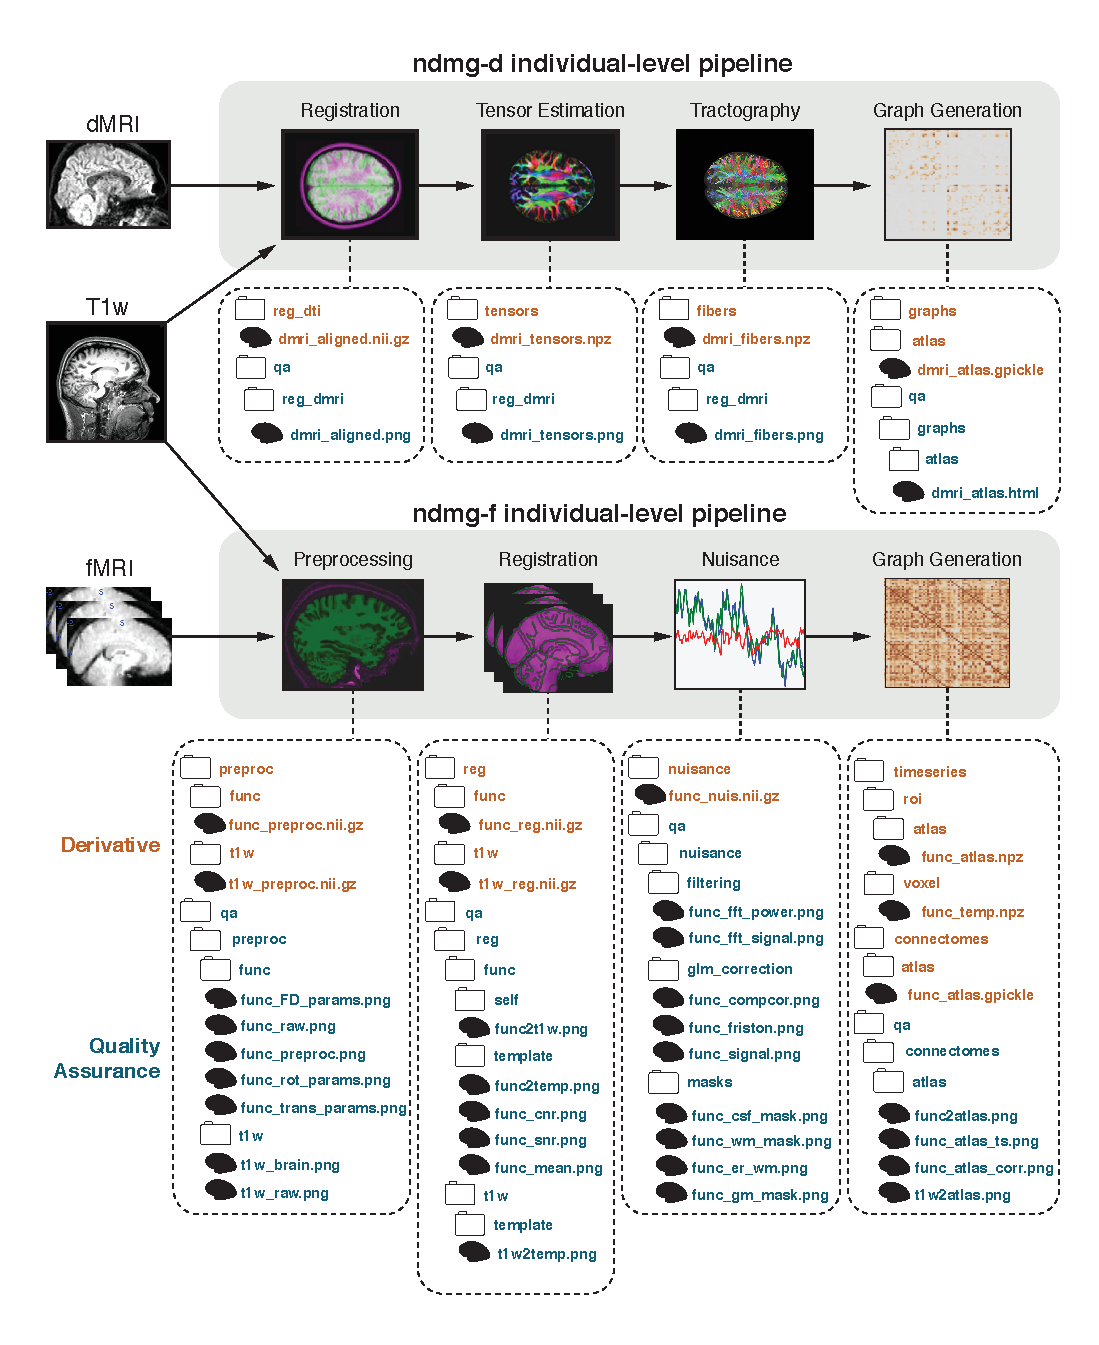
\includegraphics[width=0.9\textwidth]{./figs/ndmg_pipeline.pdf}
    \caption{\textbf{Individual Level Pipeline}
  The individual-level  \ndmg~pipeline has two sub-pipelines:  (1) \ndmgd~transforms raw dMRI data into sparse structural connectomes, and (2) \ndmgf~transforms raw fMRI data into dense functional connectomes.  Each sub-pipeline consists of four key steps, and each step generates both data derivatives and quality assurance figures to enable both qualitative assessments and quantitative comparisons (see~\ref{app:dpipe} and~\ref{app:fpipe} for details).  
%  as seen in the top. \ndmgd~consists of four main steps: registration, tensor estimation, tractography, and graph generation. Simiarly, the subject-level of the \ndmgf~pipeline transforms raw functional MRI data into structural connectomes, as seen in the bottom. \ndmgf~consists of four main steps: preprocessing, registration, nuisance-correction, and graph generation.
%  At each stage, \ndmg~produces both data derivatives and quality assurance figures of the derivative, as illustrated.
}
	\label{fig:ndmgpipeline}
\end{figure*}
%%%%%%%

%%%%%%%
%\begin{table*}
    \centering
    \caption{\textbf{\ndmg~pipeline robustness and reliability.}
We ran \ndmg~on over 20 different studies, including both fMRI and dMRI data, spanning multiple different scanners, acquisition parameters, and population demographics. Nonetheless, for both fMRI and dMRI data, across all datasets with multiple measurements, \ndmg~always achieved $>0.8$ discriminability, and \ndmgd's discriminability was typically $>0.98$ on the dMRI data. MM computes discriminability using multi-modal data from both the dMRI and fMRI connectomes. $D$=discriminability. Scanners are G (GE), P (Phillips), or S (Siemens).	
}
    \label{tab:data}
    \pgfplotstabletypeset[
    	header=true,
        string type,
        font=\addfontfeature{Numbers={Monospaced}}\small,
        columns/dset/.style={column name=Study, column type={p{.115\textwidth}}},
        columns/sca/.style={column name=Scanner, column type={p{.064\textwidth}}},
        columns/age/.style={column name={Age$\pm$1 std}, column type={p{.106\textwidth}}},
        columns/male/.style={column name=$\%$ Male, column type={p{.06\textwidth}}},
        columns/subjs/.style={column name=Indiv., column type={p{.055\textwidth}}},
        columns/ses/.style={column name=Ses., column type={p{.04\textwidth}}},
        columns/totd/.style={column name=\#Scans, column type={p{.049\textwidth}}},
        columns/trtd/.style={column name=$D$, column type={p{.048\textwidth}}},
        columns/totf/.style={column name=\#Scans, column type={p{.06\textwidth}}},
        columns/trtf/.style={column name=$D$, column type={p{.048\textwidth}}},
        columns/totm/.style={column name=\#Scans, column type={p{.049\textwidth}}},
        columns/trtm/.style={column name=$D$, column type={p{.048\textwidth}}},
        every head row/.style={
            before row={
            	\topline
                \rowcolor{tableheadcolor}
            },
            after row={\midtopline}
        },
        every odd row/.style={
        	before row={\rowcolor{vlgray}}
        },
        every row no 25/.style={
            before row={\topline\rowcolor{tableheadcolor}}
        },
        every last row/.style={
            before row={\rowcolor{tableheadcolor}},
            after row=\bottomline
        },  
        col sep=&,
        row sep=\\
    ]{dset & subjs & ses & totd & trtd \\
    HNU1    & 30   & 10 & 300  & 0.993  \\
    BNU1    & 57   & 2  & 114  & 0.984 \\
    SWU4    & 235  & 2  & 454  & 0.884 \\
    BNU3    & 48   & 1  & 47   & NA \\
    Kirby21 & 21   & 2  & 42   & 1.0 \\
    NKI1    & 24   & 2  & 40   & 0.984 \\
    Temp114 & 114  & 1  & 114  & NA  \\
    NKI-ENH & 198  & 1  & 198  & NA  \\
    Temp255 & 255  & 1  & 253  & NA \\
    PING    & 932  & 1-5& 1486 & NA \\
    MRN1313 & 1313 & 1  & 1299 & NA\\
    Pooled dMRI & 3227 & & 4347& 0.979 \\
    }
\end{table*}

\begin{table*}
    \centering
    \caption{\textbf{\ndmg~pipeline robustness and reliability.}
We ran \ndmg~on over 20 different studies, including both fMRI and dMRI data, spanning multiple different scanners, acquisition parameters, and population demographics. Nonetheless, for both fMRI and dMRI data, across all datasets with multiple measurements, \ndmg~always achieved $>0.8$ discriminability, and \ndmgd's discriminability was typically $>0.98$ on the dMRI data. MM computes discriminability using multi-modal data from both the dMRI and fMRI connectomes. $D$=discriminability. Scanners are G (GE), P (Phillips), or S (Siemens).	
}
    \label{tab:data}
    \pgfplotstabletypeset[
    	header=true,
        string type,
        font=\addfontfeature{Numbers={Monospaced}}\small,
        columns/dset/.style={column name=Study, column type={p{.115\textwidth}}},
        columns/sca/.style={column name=Scanner, column type={p{.064\textwidth}}},
        columns/age/.style={column name={Age$\pm$1 std}, column type={p{.106\textwidth}}},
        columns/male/.style={column name=$\%$ Male, column type={p{.06\textwidth}}},
        columns/subjs/.style={column name=Indiv., column type={p{.055\textwidth}}},
        columns/ses/.style={column name=Ses., column type={p{.04\textwidth}}},
        columns/totd/.style={column name=\#Scans, column type={p{.049\textwidth}}},
        columns/trtd/.style={column name=$D$, column type={p{.048\textwidth}}},
        columns/totf/.style={column name=\#Scans, column type={p{.049\textwidth}}},
        columns/trtf/.style={column name=$D$, column type={p{.048\textwidth}}},
        columns/totm/.style={column name=\#Scans, column type={p{.06\textwidth}}},
        columns/trtm/.style={column name=$D$, column type={p{.048\textwidth}}},
        every head row/.style={
            before row={
            	\topline
                \rowcolor{tableheadcolor}
            },
            after row={\midtopline}
        },
        every odd row/.style={
        	before row={\rowcolor{vlgray}}
        },
        every row no 25/.style={
            before row={\topline\rowcolor{tableheadcolor}}
        },
        every last row/.style={
            before row={\rowcolor{tableheadcolor}},
            after row=\bottomline
        },  
        col sep=&,
        row sep=\\
    ]{dset & subjs & ses & totf & trtf \\
    HNU1     &  30  & 10 & 300 & 0.956  \\
    BNU1     & 57   & 2  & 108 & 0.906  \\
    SWU4     & 235  & 2  & 466 & 0.891  \\
    BNU3     & 48   & 1  & 47  & NA  \\
    IPCAS6   & 2    & 9  & 18  & 0.994 \\
    IPCAS8   & 13   & 2  & 26  & 0.958  \\
    SWU1     & 20   & 3  & 60  & 0.935  \\
    IPCAS5   & 22   & 2  & 44  & 0.819 \\
    SWU3     & 23   & 2  & 46  & 0.986 \\
    XHCUMS   & 23   & 5  & 115 & 0.823 \\
    UWM      & 25   & 2  & 50  & 0.849 \\
    NYU1     & 25   & 3  & 75  & 0.931 \\
    SWU2     & 27   & 2  & 54  & 0.874 \\
    IPCAS1   & 30   & 2  & 60  & 0.893 \\
    IPCAS2   & 34   & 2  & 68  & 0.868 \\
    IBATRT   & 36   & 2  & 50  & 0.974 \\
    MRN1     & 52   & 2  & 90  & 0.859 \\
    BNU2     & 61   & 2  & 121 & 0.863 \\
    }
\end{table*}
%%%%%%%

In the individual-level analysis, each individual  undergoes some number of sessions, during which multiple different modalities can be collected.
The input to \ndmg~for a given individual is  the collection of scans and some metadata for each scan, including a structural scan, % (T1w/MPRAGE), 
and either, or both of, (1) a diffusion scan, including the diffusion parameters files,  and (2) a functional scan, including the slice acquisition sequence.
The individual-level of \ndmg~ analysis leverages existing open source tools, including
the fMRI Software Library (FSL) ~\cite{fsl1, fsl2, fsl3}, Dipy~\cite{dipy}, the MNI152 atlas~\cite{mni152}, and a variety of parcellations defined in the MNI152 space~\cite{desikan, aal, jhu, harvardoxford, talairach, slab907, slab1068, pvt, glasser} (see \ref{app:parcels} for details about built-in parcellations included). 
% @reb: vince says: [hey, we have a number of ICA parcellation schemes, the way we like to use them is to run spatially constrained ICA on new data using these as priors...if you want to do something with this let me know, possible collaboration going forward? ;-) ] let's get them in our set?
All algorithms requiring hyper-parameter selection were initially set to the suggested parameters for each tool, and tuned to improve the accuracy, reliability, expediency, and robustness of the results.
The output of each processing stage includes data derivatives and QA figures to enable individualized accuracy assessments.
The QA figures at many stages include cross-sectional images at different depths in the three canonical planes (sagittal, coronal, and axial) of images or overlays. Example QA figures are provided in \ref{app:dpipe} and \ref{app:fpipe}.
%---which we refer to as QAX---as specified below.
%A crucial component of the design of \ndmg~was to include  quality assurance (QA) figures for each stage to the pipeline, to enable users to easily detect whether or not the pipeline is producing accurate results. 
%Snapshots of these QA figures are shown Figure~\ref{fig:ndmgpipeline}.%, whereas exemplars are provided in \ref{app:pipeline}.

\paragraph{Individual-Level Diffusion Analysis}

The \ndmgd~pipeline consists of four key components: (1) registration, (2) tensor estimation, (3) tractography, and (4) graph generation (see Figure~\ref{fig:ndmgpipeline} for an illustration, and 
\ref{app:dpipe} for further details). It was optimized on the Kirby21 dataset, and then applied to the remaning 10 datasets.
Below, we provide a brief description of each step.

\begin{description}[style=unboxed,leftmargin=0cm]
        \item[Registration] uses FSL's ``standard'' linear registration pipeline % \textit{eddy\_correct}, \textit{epi\_reg}, \textit{flirt}, and \textit{apply\_xfm} 
        to register the structural and diffusion images to the MNI152 atlas~\cite{fsl1,fsl2,fsl3,mni152}. Nonlinear registration, though possibly more accurate~\cite{klein,lddmm}, was not sufficiently robust to include (it often failed on some studies without manual intervention).
    
        %QAX overlays of the dMRI image and the MNI152 atlas.

        \item[Tensor Estimation] uses DiPy~\cite{dipy}
%       's gradient-table, TensorModel, fit, get-sphere, and quantize-evecs
        to obtain an estimated tensor in each voxel. %QAX depicts a fractional anisotropy map.
        \item[Tractography] uses DiPy's \textit{EuDX}~\cite{eudx}, a deterministic tractography algorithm closely related to \textit{FACT}~\cite{fact}, to obtain a streamline from each voxel. %QAX visualizes of a subset of the streamlines within the MNI152 brain.
        Probabilistic tractography, while possibly more accurate, requires orders of magnitude more computational time.  Visual QA of the generated fibers suggested that deterministic was sufficiently accurate for our purposes. 
        \item[Graph Generation] Graphs are formed by contracting fiber streamlines \ref{app:graphgen} into sub-regions depending on spatial ~\cite{glocal} proximity or neuro-anatomical ~\cite{aal, desikan, harvardoxford, talairach, jhu, glasser, pvt, slab907, slab1068} similarity. QA are performed as in the functional pipeline,  described below.
%       Connectomes are created by tracing fibers through pre-defined parcellations.
%As fibers are traced, an undirected edge is added to the graph for every pair of regions along the path, where the weight of the edge is the cumulative number of fibers between two regions. 
\end{description}



%\subparagraph{Registration}
%
%\ndmgd~leverages FSL~\cite{fsl1,fsl2,fsl3} for a series of linear registrations. Taking as input the minimally preprocessed dMRI and T1W images, the end result is the dMRI volumes aligned to the MNI152 atlas~\cite{mni152}. 
%The registration pipeline implemented is ``standard'' when working with diffusion data and FSL's tools.
%The QA figure produced at this stage is cross-sectional images at different depths in the three canonical planes (sagittal, coronal, and axial) of an overlay of the dMRI image and the MNI152 atlas.
%
%\paragraph{Tensor Estimation}
%A voxelwise tensor image from the dMRI image stack using a simple 6-component tensor model from  Dipy~\cite{dipy}.
%The aligned diffusion volumes and b-values/b-vectors files are transformed into a 6-dimensional tensor volume, a single dimension \ndmg~pipeline enables three tiers of analysis: individual-level, group-level, and meganalysis (see 
%Figure for each component of the resulting tensors.
%A fractional anisotropy map of the tensors is provided for QA, again using multiple depths in each of the three canonical image planes.
%
%\paragraph{Tractography}
%Streamlines are generated from the tensors using Dipy's EuDX~\cite{eudx}, a deterministic tractography algorithm closely related to FACT~\cite{fact}.
%Each voxel within the tensor image, confined to the boundary of the brain mask, is used as a seed-point in EuDX and fibers are produced and then pruned based on their length.
%\ndmgd~provides a QA plot visualizing a subset of the generated streamlines within a mask of the MNI152 brain so that the user can verify that their structure resembles that of the fractional anisotropy map generated in the previous step.
%
%\paragraph{Graph Generation}


%Below we provide a brief description of each step, \ref{app:pipeline} provides further details.
%While each of these steps is described here, an in-depth look at the specific models and algorithms implemented at each stage contained within \ref{app:pipeline}.
Individual-level analysis in \ndmgd~takes approximately $1.5$ hours to complete using 1~CPU core and 12~GB of RAM at 1 mm$^3$ resolution.
The individual-level analysis was run on 11 studies, including 3,227 individuals and 4,347 scans. Each dataset generated connectomes across each of the parcellations in \ref{app:parcels}, resulting in 104,328 functional brain-graphs.


\paragraph{Individual-Level Functional Analysis}

The \ndmgf~pipeline can be broken up into four key components: (1) preprocessing, (2) registration, (3) nuisance correction, and (4) graph generation (see Figure~\ref{fig:ndmgpipeline}for an illustration and  \ref{app:fpipe} for further details).
The \ndmgf~pipeline was constructed starting with the optimal processing pipeline identified in Wang et. al~\cite{discriminability} using CPAC~\cite{cpac}. Hyperparameters and further algorithm selection was optimized for reliability based on multiple measurement studies (including test-retest).
Below, we provide a brief description of each step.
%, and \ref{app:fpipe} provides further details.
%While each of these steps is described here, an in-depth look at the specific models and algorithms implemented at each stage contained within \ref{app:pipeline}.

\begin{description}[style=unboxed,leftmargin=0cm]
        \item[Preprocessing] uses AFNI~\cite{AFNI}  for brain extraction, and FSL~\cite{Jenkinson2002,Woolrich2009} for slice-timing and motion correction. 
        \item[Registration] uses FSL~\cite{fsl1, Greve2009,Andersson2007}  to perform a non-linear boundary based registration of the fMRI into the MNI152 space~\cite{mni152}. 
The registration pipeline implemented is ``standard'' when working with functional data and FSL's tools~\cite{cpac}.
%QAX includes various overlays and signal-to-noise images.
%between the fMRI image and the T1w image, and the T1w image with the segmented white-matter used mask for boundary-based registration. 
%During template-alignment, QAX overlays  fMRI image and the MNI152 atlas \cite{mni152} and the T1w image and the MNI152 atlas \cite{mni152}. Additionally, QAX includes voxel-wise signal-to-noise, contrast-to-noise, and mean-intensity images.
\item[Nuisance Correction] uses custom Python code to implement a general linear model incorporating regressors for quadratic detrending \cite{Tanabe, Smith1999}, top five white-matter and cerebrospinal fluid Principal Components (CompCor) \cite{Behzadi2007,Ciric2017174}, and the Friston 24-parameter regressors \cite{Friston1996}. Low-frequency drift is then removed below $0.01$ Hz \cite{Lindquist2009}, and the first 15 seconds of the fMRI sequence are discarded \cite{Bright2016}. 
% @reb: vince says: typically there is a low pass filter applied as well, cutoff somewhere between 0.08 and 0.15.  
% @reb: let's check low-pass fileter post submission.  please add to github? or asana? i think maybe github for pipeline changes?  post in the appropriate place and delete comment here.
\item[Graph Generation] uses custom Python code to compute the average timeseries for all voxels within an ROI, then computes correlations between all pairs of ROIs. 
% @reb: vince says try ICA here, let's add ICA atlas post submission.  
%The resulting $4-d$ functional volume is masked by the MNI152 template \cite{mni152}, and the included voxels are output as the voxel timeseries. Region-of-Interest (ROI) timeseries are created by averaging the intensities of all voxels segmented into a region at each timestep. Regions are delineated by pre-defined parcellations using the same collection as \ndmgd. Correlation matrices are then created by taking the pairwise correlation between each pair of ROI timeseries. 
The functional connectome is then rank-transformed by replacing the magnitude of the correlation with its relative rank, from smallest to largest~\cite{discriminability}.  
%QA for each parcellation pipeline includes the registered functional volume overlaid with the parcellation, the registered t1w image overlaid with the parcellation, the the ROI timeseries per-ROI, and the estimated functional connectome as an adjacency matrix, and  the same graph statistics as for the diffusion connectomes. 
\end{description}


Individual-level analysis in \ndmgf~takes approximately 20~minutes to complete using 1~CPU core and 3~GB of RAM at 2 mm$^3$resolution.
The individual-level analysis was run on 714 individuals with 1,646 scans from 18 studies, generating connectomes across each of the 24 parcellations in \ndmgd, and resulting in 39,504 total brain-graphs.

\paragraph{Multi-Scale Multi-Connectome Analysis}

For both diffusion and functional MRI, \ndmg~downsamples the voxel-wise graphs to obtain weighted graphs for many different parcellation schemes. This includes: (1) neuroanatomically delineated parcellations, such as the HarvardOxford cortical and sub-cortical atlases~\cite{harvardoxford}, the JHU~\cite{jhu}, Talairach~\cite{talairach}, Desikan~\cite{desikan}, and AAL~\cite{aal} atlases; (2) algorithmically delineated parcellations, such as Slab907~\cite{slab907}, Slab1068~\cite{slab1068}, and CC200~\cite{cpac};  and (3) 16 down-sampled parcellations ranging from 70 to 72,783 nodes~\cite{glocal}.  
For each, the \emph{multi-connectome} is defined by the set of nodes from a particular parcellation, and the set of (potentially weighted and/or directed) edges from each modality.

The QA for graph generation includes a heat map of the adjacency matrix, the number of non-zero edges, and several multivariate graph statistics (one statistic per vertex in the graph) including:  betweenness centrality, clustering coefficient, hemisphere-separated degree sequence, edge weight, eigenvalues of the graph laplacian, and locality statistic-1~\cite{glocal}.
We developed the hemisphere-separated degree sequence to indicate the ipsilateral and contralateral degree for each vertex, which we found quite useful for QA.  
\ref{app:graphgenf} includes definitions and implementation details for each of the statistics.
Supplementary Figure ~\ref{fig:multiscale} shows, for a single individual, the graph summary statistics for the multi-connectome (including both functional and diffusion) across the set of atlases described above.
% @reb: post submission, consider overlaying the D & F plots 

%%%%%%%
\begin{table*}
    \centering
    \caption{\textbf{\ndmg~pipeline robustness and reliability.}
We ran \ndmg~on over 20 different studies, including both fMRI and dMRI data, spanning multiple different scanners, acquisition parameters, and population demographics. Nonetheless, for both fMRI and dMRI data, across all datasets with multiple measurements, \ndmg~always achieved $>0.8$ discriminability, and \ndmgd's discriminability was typically $>0.98$ on the dMRI data. MM computes discriminability using multi-modal data from both the dMRI and fMRI connectomes. $D$=discriminability. Scanners are G (GE), P (Phillips), or S (Siemens).	
}
    \label{tab:data}
    \pgfplotstabletypeset[
    	header=true,
        string type,
        font=\addfontfeature{Numbers={Monospaced}}\small,
        columns/dset/.style={column name=Study, column type={p{.115\textwidth}}},
        columns/sca/.style={column name=Scanner, column type={p{.06\textwidth}}},
        columns/age/.style={column name={Age$\pm$1 std}, column type={p{.106\textwidth}}},
        columns/male/.style={column name=$\%$ Male, column type={p{.06\textwidth}}},
        columns/subjs/.style={column name=Indiv., column type={p{.055\textwidth}}},
        columns/ses/.style={column name=Ses., column type={p{.04\textwidth}}},
        columns/totd/.style={column name=\#Scans, column type={p{.049\textwidth}}},
        columns/trtd/.style={column name=$D$, column type={p{.048\textwidth}}},
        columns/totf/.style={column name=\#Scans, column type={p{.049\textwidth}}},
        columns/trtf/.style={column name=$D$, column type={p{.048\textwidth}}},
        columns/totm/.style={column name=\#Scans, column type={p{.049\textwidth}}},
        columns/trtm/.style={column name=$D$, column type={p{.048\textwidth}}},
        every head row/.style={
            before row={
            	\topline
                \rowcolor{tableheadcolor}
                & & & & & &\multicolumn{2}{c}{dMRI} & \multicolumn{2}{c}{fMRI} & \multicolumn{2}{c}{MM} \\
                \rowcolor{tableheadcolor}
            },
            after row={\midtopline}
        },
        every odd row/.style={
        	before row={\rowcolor{vlgray}}
        },
        every row no 25/.style={
            before row={\topline\rowcolor{tableheadcolor}}
        },
        every last row/.style={
            before row={\rowcolor{tableheadcolor}},
            after row=\bottomline
        },  
        col sep=&,
        row sep=\\
    ]{dset & sca & age & male & subjs & ses & totd & trtd & totf & trtf & totm & trtm \\
    HNU1~\cite{corr} & G & 24.4 $\pm$ 2.3 & 0.50 & 30  & 10 & 300 & 0.993 & 300 & 0.956 & 300 & .993 \\
    BNU1~\cite{corr} & S & 23.0 $\pm$ 2.3 & 0.53 & 57  & 2  & 114 & 0.984 & 108 & 0.906 & 108 & .990 \\
    SWU4~\cite{corr} & S & 20.0 $\pm$ 1.3 & 0.51 & 235 & 2 & 454 & 0.884 & 466 & 0.891 & 452 & .903 \\
    BNU3~\cite{corr} & S & 22.5 $\pm$ 2.1 & 0.50 & 48 & 1 & 47 & NA & 47 & NA  & 47 & NA \\
    Kirby21~\cite{Kirby21}  & P  & 31.8 $\pm$ 9.4 & 0.52 & 21 & 2 & 42 & 1.0 & -- & -- & -- & -- \\
    NKI1~\cite{corr} & S & 34.4 $\pm$ 12.8 & 0.0 & 24 & 2 & 40 & 0.984 & -- & --& -- & -- \\
    Temp114 & S & 21.8 $\pm$ 3.0 & 0.58 & 114 & 1 & 114 & NA & -- & --& -- & -- \\
    NKI-ENH~\cite{nkirs} & S & 42.5 $\pm$ 19.6 & 0.40 & 198 & 1 & 198 & NA & -- & --& -- & -- \\
    Temp255 & S & 22.1 $\pm$ 3.9 & 0.51 & 255 & 1 & 253 & NA & -- & --& -- & -- \\
    PING~\cite{ping} & G/S/P & 11.7 $\pm$ 5.0 & 0.52 & 932 & 1-5 & 1486 & NA &-- &  --& -- & -- \\
    MRN1313 & S  & 27.6 $\pm$ 13.3 & 0.60 & 1313 & 1 & 1299 & NA &-- &  -- & --  & --\\
    IPCAS6~\cite{corr} & S & 23.0 $\pm$ 2.0 & 0.5 & 2 & 9 & -- & -- & 18 & 0.994& -- & -- \\
    IPCAS8~\cite{corr} & S & 57.6 $\pm$ 3.6 & 0.46 & 13 & 2 & -- & -- & 26 & 0.958 & --  & -- \\
    SWU1~\cite{corr} & S & 21.6 $\pm$ 1.7 & 0.3 & 20 & 3 & -- & -- & 60 & 0.935 & --  & -- \\
    IPCAS5~\cite{corr} & S & 18.3 $\pm$ 0.5 & 1.0 & 22 & 2 & -- & -- & 44 & 0.819 & --  & --\\
    SWU3~\cite{corr} & S & 20.4 $\pm$ 1.6 & .35 & 23 & 2 & -- & -- & 46 & 0.986 & -- & -- \\
    XHCUMS~\cite{corr} & S & 52.0 $\pm$ 6.3 & 0.60 & 23 & 5 & -- & -- & 115 & 0.823 & -- & --\\
    UWM~\cite{corr} & G & 25.0 $\pm$ 3.2 & 0.56 & 25 & 2 & -- & -- & 50 & 0.849 & -- & -- \\
    NYU1~\cite{corr} & S & 29.4 $\pm$ 8.4 & 0.4 & 25 & 3 & -- & -- & 75 & 0.931 & -- & -- \\
    SWU2~\cite{corr} & S & 21.0 $\pm$ 1.6 & 0.33 & 27 & 2 & -- & -- & 54 & 0.874 & -- & --\\
    IPCAS1~\cite{corr} & S & 20.9 $\pm$ 1.7 & 0.3 & 30 & 2 & -- & -- & 60 & 0.893 & -- & --\\
    IPCAS2~\cite{corr} & S & 13.4 $\pm$ 0.9 & 0.35 & 34 & 2 & -- & -- & 68 & 0.868 & -- & --\\
    IBATRT~\cite{corr} & S & 28.0 $\pm$ 7.5 & 0.54 & 36 & 2 & -- & -- & 50 & 0.974 & -- & --\\
    MRN1~\cite{corr} & S & 15.1 $\pm$ 7.8 & 0.5 & 52 & 2 & & & 90 & 0.859 & -- & --\\
    BNU2~\cite{corr} & S & 20.9 $\pm$ .9 & 0.54 & 61 & 2 & -- & -- & 121 & 0.863 & -- & --\\
    Pooled dMRI & & & & 3227 & & 4347 & 0.979 & -- & -- & -- & --\\
    Pooled fMRI & & & & 763 & &  -- & -- & 1798 & 0.881 & -- & --\\
    Pooled MM & & & & 361 & & -- & -- & -- & -- & 907 & 0.982 \\
    }
\end{table*}
%%%%%%%

\subsection{Group-Level Analysis}

We ran \ndmg~on the 11 diffusion and 18 functional studies listed in 
Table~\ref{tab:data}.
For each, \ndmg~group-level analysis computes and plots group-level graph summary and reliability statistics. 

%%%%%%%
\begin{figure*}[b!]
\centering
\includegraphics[width=\textwidth]{./figs/fig_graphqa.pdf}
\caption{\textbf{\ndmg's group level analysis computes and plots eight connectome-specific summary statistics per modality for each scan, providing immediate quality assurance for the entire study.} In theory, any connectome could be an outlier for any of these statistics, so plotting all of them together is particularly useful (see~\ref{app:graphstats} for details). The top panels  show results for the BNU1 dMRI connectomes, the bottom panels show the results for the BNU1 fMRI connectomes.
}
\label{fig:graphqa}
\end{figure*}
%%%%%%%

\paragraph{Group Level Implementation Strategy}

Leveraging previous efforts developed in our  ``Science in the Cloud''~\cite{sic} manuscript, multiple scans and studies are evaluated in parallel for participant-level analysis, and the derivatives are pooled for group-level analysis, much like typical map-reduce approaches (consistent with the BIDS app specification~\cite{bidsapps}). The parallel  implementation uses the Amazon Web Services (AWS) cloud, in particular leveraging their storage (S3) and high performance computing (Batch) services. Data are stored in an S3 bucket enabling  the \ndmg~cloud-API connectome estimation pipeline to process all scans on Amazon Batch in parallel. In practice,  AWS limits the number of parallel threads users are allowed to launch (to prevent accidental spending). After connectome estimation is complete, the same cloud-API exposed by \ndmg~enables group-level analysis to be launched and parallelized across each parcellation for all scans within each study.
% 
% > our
% or "the"
% 
% ^.
We were able to compute diffusion connectomes at 24~scales for each of the publicly available 2,861~scans (totaling 68,664~connectomes) in under one day and \$1,000. Had we processed each scan in parallel, cost would have remained the same but only taken $1.5$~hours.

\paragraph{Group-Level Graph Summary Statistics}

Each scan's estimated connectome can be summarized by a set of graph statistics, as described above. For group-level analysis, we visualize each scan's summary statistics overlaid on one another. For example, Figure~\ref{fig:graphqa} demonstrates that each diffusion graph from the BNU3 dataset using the Desikan atlas has relatively similar values for the statistics (we use the Desikan atlas for the remainder of the analyses unless otherwise specified). Moreover, it is clear from both the degree plot and the mean connectome plot that the dMRI connectomes from this study tend to have more connections within a hemisphere than across a hemisphere, as expected. For the fMRI connectomes, however, the homotopic connections---that is, connections from one region on a hemisphere to the same region on the other hemisphere---seem particularly strong.
%Supplementary Figure ~\ref{fig:graphqaf} shows example group-level analysis for the same study's functional data.
 
%\ref{app:multi} illustrates how \ndmg~also computes the average value for each univariate and multivariate statistic for each atlas, and demonstrates similarities across scales, indicating that that the basic structure of the connectomes is preserved across different atlases.


%\subsubsection{\ndmgf~Individual-Level Pipeline}

\paragraph{Group-Level Discriminability}
\label{sec:disc}

Group-level results from \ndmg~that include repeated measurements are quantitatively assessed using a statistic called discriminability~\cite{discriminability}.
The group's sample discriminability estimates the probability that two observations within the same class are more similar to one another than to objects belonging to a different class:
\begin{equation}
D = Pr(|| a_{ij} - a_{ij'} || \leq || a_{ij} - a_{i'j'} ||).
\label{eq:disc}
\end{equation}
In the context of reliability in \ndmg, each connectome, $a_{ij}$, is compared to other connectomes belonging to the same individual, $a_{ij'}$, and to all connectomes belonging to other individuals, $a_{i'j'}$.
A perfect discriminability score indicates that for all observations within the group, each connectome is more like connectomes from the same individual than others.
Table~\ref{tab:data} lists the discriminability score of each study with repeated measurements (five dMRI studies and sixteen fMRI).
 \ndmgd~achieves a discriminability score of nearly 0.99 or greater on most studies (the lowest score was nearly 0.9).  \ndmgf~achieves a discriminability score around 0.9 on all studies. 
These high discriminability scores  were achieved by optimizing both \ndmgd~and \ndmgf~on a subset of the data.  Specifically, \ndmgd~was optimized using only the Kirby21 study, to achieve a perfect discriminability score.  Nonetheless, the other studies achieved comparably high discriminability scores, despite the fact that the Kirby21 used a Philips scanner, unlike any of the other studies. Moreover, Kirby21's age distribution is substantially different from several of the other dMRI studies (see Table~\ref{tab:data}).  
Similarly, \ndmgf~was optimized using only 13 of the 18 studies, and yet discriminability on the remaining studies remained equally high~\cite{discriminability}, even though they also exhibited large study demographic and acquisition protocol variability.
Finally, \ndmg~was not optimized explicitly at all on multimodal data, nonetheless, for all datasets with multiple scans per subject with both dMRI and fMRI, using the multimodal connectomes improved (or did not decrease) discriminability relative to either modality on its own.
That \ndmg's discriminability score is robust to data acquisition details and study demographics across modalities suggests that scientific results may also be robust to such sources of variability.

% Note that we invested significant effort in both pipelines to achieve these high discriminability scores, and to our knowledge, no other pipelines have been assessed with regards to discriminability. 
 
 % or any other reliability metric.
%
%The discriminability score obtained if a pipeline produced random outputs is summarized in Equation~\ref{eq:chance}, and is a function of the number of classes, $k$, the number of elements in each class, $M_i$, and the total number of observations, $N$:
%
%\begin{equation}
%C = \frac{\sum_{i \in k}^{k}M_{i}^{2}}{N^{2}}.
%\label{eq:chance}
%\end{equation}
%
%Optimizing \ndmg~with respect to discriminability enables us to minimize the upper-bound on error for any general downstream inference task.
%Using discriminability for optimization also prevents over-fitting to covariate-specific signal (i.e. in contrast to optimizing the pipeline for sex classification).

\subsection{Mega-Level Analysis}

Many sources of variability contribute to the observed summary statistics, including individual- or population-level variation,  and different types of measurement or analysis techniques. By virtue of harmonizing the analysis across individuals and studies, we are able assess the remaining degrees of variability due to measurement and demographic-specific effects. Although population-level effects are expected when comparing two different populations with different demographics, variability across measurements must be relatively small for inferences based on neuroimaging to be valid across these populations. Therefore, we conducted mega-analysis to address these remaining sources of variation.  


\paragraph{Consistency Within and Across Studies}

%%%%%%%
\begin{figure*}[t!]
\centering
\begin{subfigure}[h]{\textwidth}
\includegraphics[width=\textwidth]{./megamean/megamean.png}
\end{subfigure}
\caption{\textbf{Multi-Study Mean Connectomes}. 
Site-specific mean connectomes (top two rows) and mega-mean (bottom row), using the Desikan parcellation, 
%Dataset-mean connectomes and a combined mean-of-mean Desikan labeled graphs 
%produced by \ndmg, 
%resulting in the largest
%known mean connectome to-date, 
using all the data for which we have both functional and diffusion studies ($>900$ scans of each), with edges and vertices colored depending on hemisphere.
%Bilateral edges connecting the same regions in opposite hemispheres are shown in black. 
In the top 2 rows, graphs are shown with vertex position determined by the coronally-projected center of mass for each region in the Desikan parcellation.  The bottom shows radial plots organized by hemisphere.
Same-modality connectomes appear qualitatively similar to one another across sites, but some differences across modalities are apparent.  For example, 
homotopic and contralateral connections both seem stronger in functional than diffusion mean connectomes, both within site and after pooling all sites.
%, ipsi-lateral connectivity in the diffusion connectomes is consistently more dense than contra-lateral
%connectivity in the functional connectomes. 
%Likewise, homotopic connectivity in the functional connectomes appears more dense than heterotopic connectivity in the diffusion connectomes.
}
\label{fig:mean}
\end{figure*}
%%%%%%


Figure~\ref{fig:mean} (top) shows the mean estimated connectome computed from each dataset for which we have both dMRI and fMRI data.  We also calculate the  mega-mean connectomes, that is, the mean derived by pooling all the studies (Figure~\ref{fig:mean}, bottom).  Several group-specific properties are readily apparent simply by visualizing the connectomes:
% @reb: nice, can you make this the default in our neurodata.sty package?
\begin{enumerate}[wide, labelwidth=!, labelindent=0pt, label=\bf{\arabic*)}]
        \item The dMRI connectomes have significantly stronger ipsilateral connections than contralateral connections, meaning connections are more prevalent within hemispheres, on average.
        \item The fMRI connectomes have significantly stronger homotopic connections than heterotopic connections, meaning region A on the left hemisphere tends to correlation with region A on the right hemisphere, more than other regions, on average. 
\end{enumerate}

To formally test these initial assessments we developed statistical connectomics models and methods. Specifically, we developed a structured independent edge random graph model that generalizes the more commonly used  stochastic block model (SBM)~\cite{Holland83} and the independence edge random graph model~\cite{Bollobas2009}. In this new model, each edge is sampled independently, but not identically. Rather, there are $K$ possible probabilities of an edge between a pair of vertices, and we have \emph{a priori} knowledge of which edges are in which groups.  Unlike the SBM 
% @jv: we need to report n and the test details more extensively here, particularly whether it is one or 2-sided (one-sided here)
 model, in which each \emph{vertex} is in a group, here each \emph{edge} is in a group.  We then developed test statistics that are consistent and efficient for this model. Specifically, with sufficiently large sample sizes, the power (the probability of correctly rejecting a false null hypothesis) of our test approaches unity for the model under consideration.  Moreover, no other test can achieve higher power with fewer samples under this model (see ~\ref{app:siem} for details).

Using the above described approach, we first quantify the degree to which ipsilateral connections tend to be stronger than contralateral connections (Figure~\ref{fig:siem}A).   
$100\%$ of dMRI connectomes and $99.4\%$ of fMRI connectomes, exhibit stronger ipsilateral than contralateral connections.
The dMRI connectomes typically have a larger difference between ipsilateral and contralateral connections, as evidenced by the magnitudes of differences (Figure ~\ref{fig:siem}A.i). and the cumulative probability of a connectome having a difference that is statistically significantly at any level (Figure ~\ref{fig:siem}A.ii).
We subsequently investigated whether for a given individual, the difference between ipsilateral and contralateral connections was stronger in the dMRI data than the fMRI data. 

Out of $907$ individuals with both dMRI and fMRI scans, $99.9\%$ exhibit  stronger ipsilateral versus contralateral connections in the dMRI scan as compared to their corresponding fMRI scan (Figure ~\ref{fig:siem}A.iii), with $99.5\%$ significant at the $0.05$ level, for example (Figure ~\ref{fig:siem}A.iv).

We applied the same strategy to test whether homotopic connections tend to be stronger than heterotopic connections (Figure~\ref{fig:siem}B). In this case, the results are essentially opposite. Here, $100\%$ of the fMRI and dMRI connectomes exhibit this property (Figure ~\ref{fig:siem}B.ii). Similarly, for nearly all individuals ($99.9\%$) with both functional and diffusion scans, the relative strength of homotopic versus heterotopic connections was stronger in his or her fMRI data than the dMRI data (Figure ~\ref{fig:siem}B.iii), with $99.0\%$ significant at the $0.05$ level (Figure ~\ref{fig:siem}B.iv).  


% @reb: post submission, get PING dataset from gkiar and analyze too
In other words, there is a marked consistency across \emph{all} individuals in \emph{all} studies (18 fMRI studies and 10 dMRI studies) for these most basic statistical properties of multi-modal connectomes. Notably, this result provides compelling evidence that certain connectomic discoveries that utilize only a single study, or even a single individual, without even addressing batch effects, can reasonably be expected to be repeatable across studies. Note, however, that repeatable does not mean correct; the true relative probabilities of ipsilateral, contralateral, homotopic, and heterotopic connections in humans remains an open question. 


%%%%%%%
\begin{figure*}[t!]
\centering
\begin{subfigure}[h]{\textwidth}
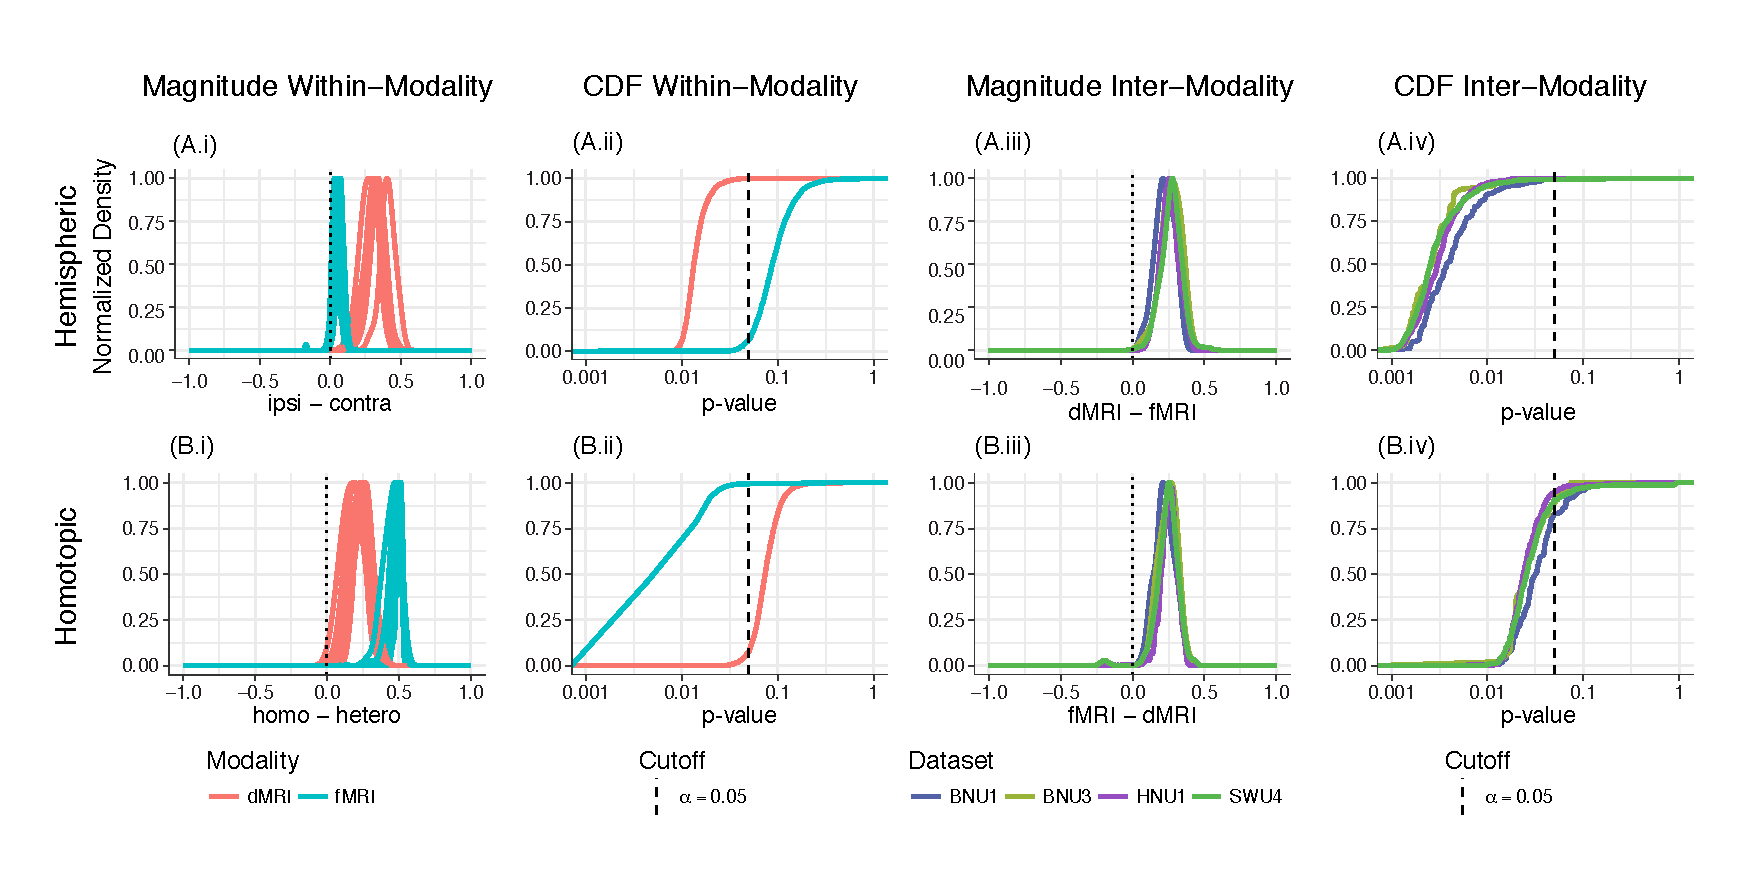
\includegraphics[width=\textwidth]{./figs/figure_siem.pdf}
\includegraphics[width=\textwidth]{./figs/table_siem.pdf}
\end{subfigure}
\caption{\textbf{Structured Independent Edge Model  (SIEM) establishes multi-connectome properties are preserved both within and across studies}.
\textbf{(A.i)} The magnitude of the difference indicating whether ipsilateral (within hemisphere) connections differ from contralateral (across hemisphere) connections. The dMRI connectomes appear to have a greater connectivity difference than fMRI connectomes.
\textbf{(A.ii)} The distribution of p-values indicating whether ipsilateral connections are significantly stronger than contralateral connections, on average.  Essentially every dMRI connectome yields significantly stronger ipsi- than contralateral connectivity, whereas essentially no fMRI connectome does.  
\textbf{(A.iii)} For four studies with both dMRI and fMRI, one can compare connection strengths across modalities for a particular individual. The ipsi-versus-contra discrepancy in the dMRI exceeds that of the fMRI.
\textbf{(A.iv)}  In essentially all sessions, dMRI has a significantly stronger within-versus-across discrepancy of connection strength than the corresponding fMRI connectome in most of same-individual pairs. 
\textbf{(B.i)} Same analysis comparing homo- to heterotopic connections, indicating that the fMRI connectomes appear to have a greater connectivity difference than the dMRI connectomes.
\textbf{(B.ii)} fMRI exhibits significantly stronger homotopic connections, whereas dMRI does not.
\textbf{(B.iii)} Same approach as (A.iii), the homo-versus-hetero discrepency in the fMRI exceeds that of the dMRI.
\textbf{(B.iv)} fMRI has a significantly stronger homo-versus-hetero discrepancy of connection strength than the  corresponding dMRI connectome. 
% of the intra-modality per-graph $p$-values that ipsi-lateral connectivity exceeds contra-lateral connectivity,  one line per site. Low $p$-values indicate that  ipsilateral connectivity is significantly stronger than contralateral.  ~\textbf{(C)} the density estimates of the inter-modality 2-graph $p$-values that this difference in connectivity is stronger in the dMRI connectomes for a particular individual than in the fMRI connectomes for that individual. One line is reported per dataset indicated in the legend. Low $p$-values indicate that we are less-likely to falsely report a difference in connectivity in dMRI connectomes vs. fMRI connectomes. $99.5\%$ of the graph-pairings exhibit this property. \textbf{(B)} the density estimates of the per-graph $p$-values that homotopic connectivity exceeds heterotopic connectivity. Low $p$-values indicate that we are less-likely to falsely report a difference in connectivity homotopically  vs. heterotopically. $99.4\%$ of the fMRI connectomes exhibit this property, whereas only $7.7\%$ of the dMRI connectomes exhibit this property. ~\textbf{(D)} the density estimates of the 2-graph $p$-values that this difference in connectivity is stronger in the fMRI connectomes for a particular individual than in the dMRI connectomes for that individual. Low $p$-values indicate that we are less-likely to falsely report a difference in connectivity in fMRI connectomes vs. dMRI connectomes. $99.0\%$ of the graph-pairings exhibit this property.
\textbf{(C)} Table showing fraction of individuals exhibiting significance effects of each analysis described above, demonstrating consistency across individuals and studies.}
\label{fig:siem}
\end{figure*}
%%%%%%%

%%%%%%%
\begin{figure*}
\begin{subfigure}[t]{\textwidth}
    \centering
	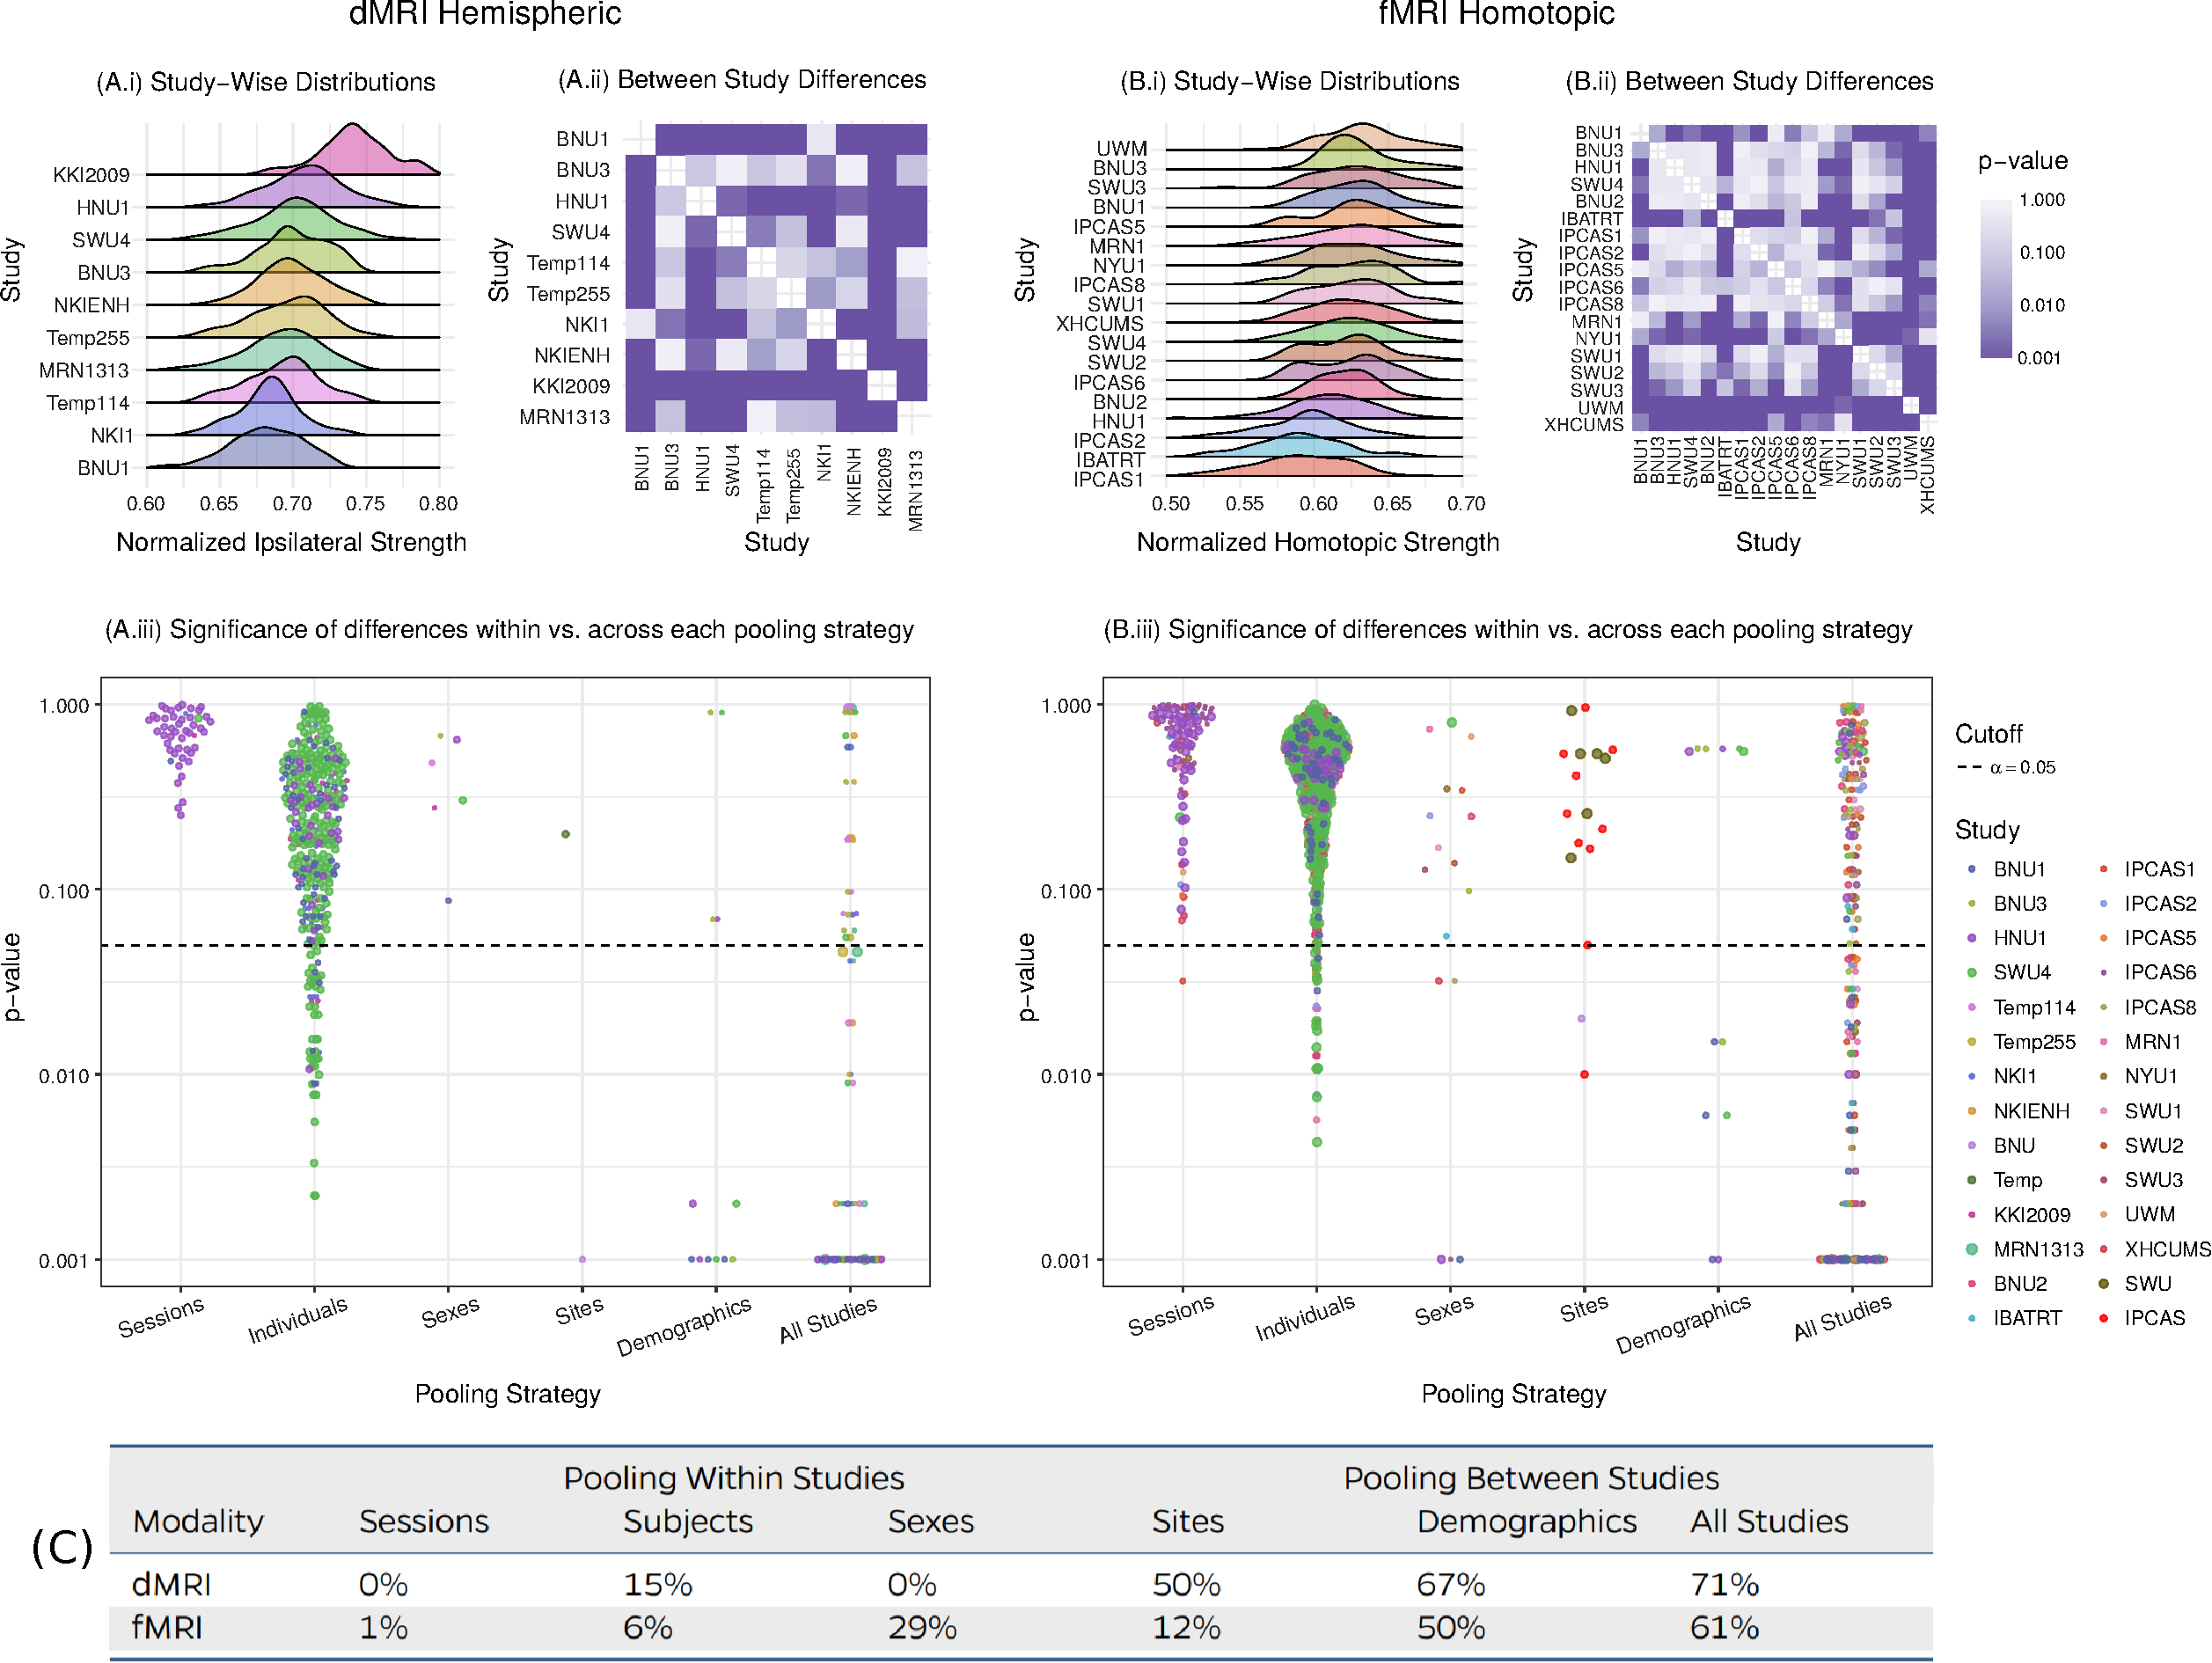
\includegraphics[width=\textwidth]{./figs/fig_batch.pdf}
\end{subfigure}
\caption{\textbf{The prevalence of connectome batch effects are investigated within and across studies using different delineations of the edges into communities for dMRI and fMRI.}
\textbf{(A)} dMRI connectomes delineate edges into within and across hemisphere. 
 \textbf{(B)} fMRI connectomes delineate edges into homotopic and heterotopic edges. 
% batch effects are instead investigated with a homotopic delineation of the vertices, with one community $C_p$ the homotopic edges and the other community $C_q$ the heterotopic vertices. The edge communities were chosen as these communities showed a significant difference in Figure (\ref{fig:siem}), indicating potential for biological signal. 
\textbf{(A.i)} and \textbf{(B.i)} Density estimates of distribution of average ipsilateral or homotopic connection strength within studies. Both within and across study variance is distressingly high.
%the model fit for the ipsi-lateral connections, where $\mathbb{E}\left[\hat{p}\right]$ is the average normalized rank of ipsi-lateral connections or homotopic connections in the dMRI connectomes and fMRI connectomes, respectively. 
\textbf{(A.ii)} and \textbf{(B.ii)} The pairwise significance of  the differences between studies demonstrates that many pairs of studies exhibit significant batch effects. 
%in a paiBatch effect is investigated between each pair of studies. Studies are arranged based on similarity of demographic, where BNU1, BNU3, HNU1, and SWU4 are placed together. $p$-value indicates the significance of a batch effect pooling between the pairs of studies. 
\textbf{(A.iii)} and \textbf{(B.iii)} Several common pooling strategies are investigated, including pooling across  \emph{sessions} within a  study, pooling across \emph{subjects} within a  study, pooling across \emph{sex} within a  study, pooling across studies  from a  scanning \emph{site}, pooling across studies with a similar basic \emph{demographics}, and pooling across \emph{all studies}. In many cases, even when controlling for these factors, significant batch effects remain.
%In each case the number of significant pairs of studies indicates 
\textbf{(C)} The fraction of samples showing significant batch effect at $\alpha = 0.05$. Pooling across sessions, subjects, and sexes,  a small fraction of the samples show significant batch effect in both the dMRI and fMRI connectomes. Pooling across demographics and across all studies  shows  large  batch effects. These results indicate that multiple (typically uncontrolled) variables considerably  impact connectome inferences, implying that  further efforts to mitigate these effects will be required to obtain sufficiently reliable estimates.
}
\label{fig:batch}
\end{figure*}

%%%%%%%

\paragraph{Significant Variability Within and Across Studies}

%At coarse resolution, each study's connectomes exhibited similar properties. However, t
While the above analysis demonstrates preservation of certain connectome properties both within and across studies, it is insufficient to determine the extent of ``batch effects''--- sources of variability including differences in participant recruitment, screening, and demographics as well as scanner, acquisition sequence, and operator.  Typically, investigators prefer that their results are robust to these additional sources of variance.
 If the batch effects are larger than the signal of interest (for example, whether a particular individual is suffering from a particular psychiatric disorder), then inferences based on individual studies are prone to be unreliable.  
%%%%%%%%
%\input{table_pipes.tex}
%%%%%%%%

Figure~\ref{fig:batch} evaluates the variability of individual scans both within and across studies for dMRI (left) and fMRI (right). For simplicity, we focus on a single parameter for each modality:  dMRI data is evaluated in terms of its average within hemisphere connectivity and fMRI is evaluated in terms of its average homotopic connectivity. Prior to analysis each graph is ``rank normalized'', meaning that its edge weights are converted into the numbers $1,2,...,N$, where $N$ is the total number of potential edges, and where the smallest value is assigned a $1$, the next smallest is assigned a $2$, etc. By virtue of this normalization, each network has the same mean and variance, therefore mitigating certain kinds of batch effects. Moreover, by partitioning edges into only two groups, there is only a single degree of freedom: the average connection strength from one group determines that of the other, and vice versa (see~\ref{app:batch} for details).
The fact that the most salient features when visualizing these connectomes effectively yields a one-dimensional characterization of this property justifies the importance of studying the batch effects of this parameter.   
Dramatic variability in this parameter suggests that more ``fine'' parameters, such as the connection strength between individual regions of interest, will typically necessarily have even greater variability.

Figure~\ref{fig:batch}(A.i) and (B.i) shows fairly dramatic variability both within and across studies, suggesting the presence of significant batch effects in both cases. Figure~\ref{fig:batch}(A.ii) and (B.ii) evaluates the statistical significance of batch effects across studies, demonstrating that many studies, though not all, do exhibit severe batch effects. In this case, batch effect was quantified by determining whether the distribution of connection strengths for one study was significantly different from those of another study.

To further understand the source of this variability, we conducted an extensive within and between study analysis of individuals, including the following six different cases (Figure~\ref{fig:batch}(A.iii) and (B.iii)):
\begin{enumerate}[wide, labelwidth=!, labelindent=0pt, label=\bf{\arabic*)}]
        \item  Across \emph{sessions} for a given individual within studies:  If  session 1  scans tended to be different from session 2 scans within a study, then the ``scan order'' itself can meaningfully impact inferences. While dMRI sessions never resulted in significant scan order effects, $9\%$ of fMRI studies were significantly impacted by this effect.   
        \item Across \emph{individuals} within studies: This analysis quantifies the fraction of individuals in a given study whose scans are less similar to one another than they are to any other scan in the dataset. $6\%$ and $15\%$ of individuals within studies (for fMRI and dMRI, respectively) have significantly different connection strengths.
        \item Across \emph{sexes} within studies: Connection strengths are the same at this coarse level across sexes for each dMRI study, whereas $30\%$ of fMRI studies demonstrated significant differences across sexes.
        \item Across studies within \emph{sites}: Two dMRI and three fMRI sites provided data from multiple studies; thus, while the location and scanner were the same across these studies, certain variability in demographic and acquisition details persisted. Both dMRI and fMRI demonstrated a mix: sometimes these differences were significant, but not always. 
        \item Across studies within \emph{demographic}: four dMRI and four fMRI studies controlled basic demographic variables,  including only Chinese people, about $50\%$ female, and all college age. Even preserving these demographics was typically insufficient to mitigate batch effects, with $2/3$ and $1/2$ of comparisons yielding significant batch effects for dMRI and fMRI, respectively.
        \item Across \emph{all} studies: 10 dMRI and 18 fMRI studies were compared, ignoring acquisition and demographic detail. Over $60\%$ of pairwise comparisons for both dMRI and fMRI demonstrated significant differences, often the maximal significance level given our permutation test.
\end{enumerate} 

Taken together, the above results indicate the existence of many difference sources of variability, even upon harmonizing analyses (Figure~\ref{fig:batch}(C)). Such variability suggests that the reproducibility of both dMRI and fMRI can benefit by further understanding, quantifying,  and mitigating these sources of variability.




\section{Discussion}


%The issues of reproducibility and batch effect spans essentially every discipline of science, although it has been particularly problematic in  omics~\cite{Leek2010-vs, Rosenfeld2010-nf, Chen2011, Nygaard2016-hw, Goh2017-hc} and more recently 
%The potential sources of variability  include
The goal of any scientific investigation is not to characterize the observed sample data’s variance, but rather, to make inferences about the general population on the basis of those data.  
Variability of sample demographics, data acquisition details (for example, number of repetitions for fMRI, number of directions for dMRI), analysis methods, measurement error, questionable research practices, or statistical errors can each contribute to limitations in generalizing to populations in psychology~\cite{Button2013} and neuroimaging~\cite{Costafreda2009}.
Our principles for pipeline development enabled a rigorous high-throughput analysis of multi-study, multi-site, and multi-connectome data to identify and quantify different sources of variability.

While perhaps seemingly at odds, the results from Figures~\ref{fig:siem} and~\ref{fig:batch} are complementary.  Specifically, Figure~\ref{fig:siem} demonstrates that essentially all connectomes share a particular property: stronger connections in one set of edges than another. On the other hand, Figure~\ref{fig:batch} demonstrates that although some sets of edges tend to be larger than others, the {magnitude} of the differences is highly variable both within and across studies. That the \emph{magnitude} of certain parameters can differ while the \emph{sign} of those parameters can be constant parallels recent suggestions from the statistics literature to move away from ``Type I'' and ``Type II'' errors, to Type M (magnitude) and Type  S (sign) errors~\cite{gelman14a}. Moreover, it suggests a strategy to understand and address batch effects: reporting the \emph{precision} for which effects are preserved or variable.  For example, in this study, when using the coarsest possible precision (larger versus smaller as in Figure~\ref{fig:siem}), no batch effects arise, whereas when using an extremely fine precision (the difference in magnitude as in Figure~\ref{fig:batch} ), batch effects are pervasive. The natural question then becomes: at which precision, for a given parameter and source of variability, do the studies still agree? Such analyses could then be incorporated into downstream analyses to preserve results across studies. 







%The \ndmg~pipeline is a reliable tool for structural and functional connectome estimation and analysis with  a low barrier to entry, and is capable of producing accurate brain-graphs across studies.
%
The design criteria for \ndmg~required certain trade-offs, including robustness under variability versus optimality under idealized data.  
% Optimizing \ndmg~for any individual dataset would make it sub-optimal for other datasets.  
Nonetheless, \ndmg, could be improved along several dimensions.
%Below we suggest several strategies that could  improve \ndmg~along various dimensions.
First, 
%several of the algorithm choices required trade-offs between accuracy and expediency, 
recent advances in registration~\cite{lddmm} and tractography ~\cite{probtrackx} could be incorporated.
When implementations for these algorithms achieve suitable expediency and robustness, it will be natural to assess them. 
Second, recently several more sophisticated batch effect strategies have been successfully employed in dMRI data~\cite{Fortin2017-dm}. Such strategies could possibly help here as well, especially if they are modified appropriately to work on binary graphs~\cite{Leek2007}.
%
Third, there is some evidence that machine learning approaches to mitigating batch effects can be effective as well, but so far only in fMRI data and only using four, rather than 18 studies~\cite{abraham2017deriving}.
Fourth, pre-processing strategies have been employed to improve multi-site reliability~\cite{mirzaalian2017harmonization}, so implementing methods such as these within \ndmg~could possibly mitigate some batch effects, at the risk of reducing accuracy and/or reliability~\cite{adhd}.
%First, several of the algorithm choices required trade-offs between accuracy and expediency, including registration~\cite{lddmm} and tractography.  When implementations for more accurate algorithms achieve suitable expediency, it will be natural to include them. 
%Second,  recently several more sophisticated batch effect strategies have been successfully employed in dMRI data~\cite{Fortin2017-dm}.  Such strategies could possibly help here as well, especially if they are modified appropriate to work on binary graphs~\cite{Leek2007,Chen2011} 
%Third, there is some evidence machine learning approaches to mitigating batch effects can be effective as well, but so far only in fMRI data and only using four, rather than 18 studies~\cite{abraham2017deriving}.
%Fourth, post-data collection stratification to harmonize study demographics has also been demonstrated to be effective to reduce batch effects of fMRI, although this study used only two studies with the same scanner~\cite{Noble2017}. 
%Pre-processing strategies have been employed to improve multi-site reliability~\cite{mirzaalian2017harmonization}, implementing  methods such as these within \ndmg~could possibly mitigate some batch effect, at the risk of reducing accuracy and/or reliability~\cite{adhd}.


%Other efforts have focused on multi-study data. Specifically, Abraham et al. \cite{abraham2017deriving}
%%Multi-site predictive tasks have been performed considering 
%used fMRI-derived connectomes from the ABIDE dataset, and demonstrate an impressive ability to minimize batch effects. Unfortunately,  most ABIDE studies lack dMRI data, so a similar strategy for \ndmgd~is not currently possible.  Similarly, concomitant with our manuscript is Noble et al. \cite{Noble2017}, who conducted a multi-scanner analysis with harmonized  fMRI acquisition on 12 individuals.  The compelling results suggest that pooling across studies with harmonized acquisition can potentially improve reliability.
%%and performing similar analyses upon a multi-dataset collection of dMRI-derived connectomes is an exciting avenue for future exploration.
%Additionally, a variety of studies propose methods for post-acquisition data harmonization using either minimally pre-processed or raw MRI data~\cite{mirzaalian2017harmonization,Fortin2017-dm,adhd} that could be explored within the context of the \ndmg~pipeline.





% \ndmg~has been optimized with respect to discriminability, yet  one can always further improve the pipeline via incorporating additional algorithms, datasets, or metrics.  For example, one could further optimize to reduce the batch effect.
%Alternately, one could incorporate probabilistic tractography to compare with deterministic approaches in a principled meganalysis using the open source data derivatives generated here.
%an exhaustive hyper-parameter sweep optimizing each parameter selection in \ndmg~has not yet been conducted.
%Though this has not occurred, an important contribution of \ndmg~is the illustration that highly sophisticated and computationally burdensome algorithms such as probabilistic tractography are not necessary to create reliable estimates of brain connectivity.
%Evaluating the quality of connectome estimation pipelines using probabilistic tractography with discriminability would enable a decisive answer to the question of when deterministic or probabilistic tractography is a more reliable when estimating connectivity, and by how much.




%Several previously proposed fMRI or dMRI pipelines utilize different algorithms which could also be incorporated, but have not been investigated here for various reasons.  CPAC~\cite{cpac}, PANDAS~\cite{Cui2013}, and CMTK~\cite{Daducci2012},   are flexible pipelines enabling users to select hyper-parameters for their dataset. This is a useful feature for many applications, but when the desire is to increase reliability, harmonization is key.
%%This freedom emphasizes the between-dataset differences in connectomes estimated with varying processing parameters, and cannot necessarily be directly compared.
% MRCAP~\cite{mrcap} and MIGRAINE~\cite{migraine} provide reference pipelines, but are difficult to deploy, and also lack vetting across studies. 
%%In the present study, we chose many pipelines for the evaluation while some existing pipelines were not included for such a purpose. 
%%Several analytic pipelines of resting-state fMRI that we did not evaluate above include
%REST~\cite{Song2011}, DPARSF~\cite{Yan2010}, DPABI~\cite{Yan2016}, GRETNA~\cite{Wang2015}, and GIFT~\cite{Calhoun2001-wc} lack command line interfaces and therefore are much more difficult to run at scale in a reliable fashion. 
%%limited to  are very popular with user-friendly graphic user interfaces (GUIs), however, it is not trivial for users to translate them into  computational platforms for  very large-scale neuroimaging data analysis. 
%Surface-based pipelines of rfMRI data such as connectome computation system (CCS)~\cite{Xu2015} and HCP (only volume-based part was included in the current evaluation) will be investigated in future work~\cite{Zuo2013}.


It may be that analysis methods on their own are insufficient to mitigate replicability issues, and that further improving data acquisition and/or data acquisition harmonization may be required. Indeed, a recent study by Noble et al.~\cite{Noble2017} found relatively few batch effects in fMRI data, although it employed only two datasets with enhanced and harmonized data acquisition protocols. 

%that post-data collection stratification to harmonize study demographics effectively to reduce batch effects of fMRI, although only in one much smaller mega-level analysis using  two studies with the same scanner.  


%However, while the algorithms that these pipelines leverage have become standard, the pipelines have not. Indeed, there is a distinct lack of reference pipelines in the field. This has resulted in each publication using  (sometimes subtly) different parameters, often without specifying  precise details and dependencies, making reproducibility difficult.  Moreover, the lack of reference pipelines also creates inefficiencies in the collective scientific process because pipelines have to be designed and tuned for each study, essentially.  


Because the methods developed herein are open source and easy to use, and the data are open access, this work enables further studies to assess measurement errors as well as variability of sample demographics and experimental protocols. For example, data could be sub-sampled to only include scans that pass stringent quality assurance standards, or have a sufficiently long duration to support discriminable connectomes~\cite{Airan17}.
% @EB: update citation.
 Alternately, this analysis could be repeated on data that is ``perfectly'' harmonized. In general, further work developing and applying experimental and theoretical tools to parse the relative impact of various sources of batch effects, as well as batch effect mitigation strategies, will be crucial for neuroimaging to achieve its greatest potential scientific and clinical value. 

%Perhaps even more problematic is that such pipelines cannot readily be used for meganalysis (an approach that pools data across datasets, centers, or studies) because most  are idiosyncratically designed for a particular study~\cite{Costafreda2009}. This stifles our ability to understand and quantify batch effects in neuroimaging, which are extremely problematic in -omics data~\cite{Leek2010-vs, Rosenfeld2010-nf, Nygaard2016-hw, Goh2017-hc}, though relatively understudied~\cite{Olivetti2012-vy, Fortin2016-yq, Fortin2017-dm}.



%The Human Connectome Project (HCP) has recently collected an extraordinary M3R dataset, and developed processing
%pipelines accordingly. It is our belief that \ndmg~is explicitly not in competition with the tools and resources
%produced by HCP. The HCP pipeline when run on the HCP data creates likely the most outstanding map of human brain
%connectivity to date, however, their pipeline relies on many additional parameters and files (such as scanner bias
%fields, and multi-shell acquisitions of dMRI data), making it unable to be deployed across the majority of existing
%dMRI studies. \ndmg~takes the approach of being a generally useful, reliable, and impactful tool, without requiring
%state-of-the-art acquisitions which are not commonly available outside of next-gen experimental paradigms. \ndmg~can be
%deployed on the HCP data, though it would not take advantage of the additional scans and parameters acquired. We
%believe that the HCP pipelines and \ndmg~compliment one another, and comparing the two more closely is an exciting
%avenue to be explored in future work.
% @rjv: I'm not sure we nd this anymore? Good to keep written when reviewers ask, though. -gk




\end{multicols}

\paragraph{Acknowledgements} 
{\small
The authors from JHU are grateful for the support  by the XDATA program of the Defense Advanced Research Projects Agency (DARPA) administered through Air
Force Research Laboratory contract FA8750-12-2-0303;  DARPA SIMPLEX
program through SPAWAR contract N66001-15-C-4041;  DARPA GRAPHS
contract N66001-14-1-4028; National Science Foundation grant 1649880, 
 and
the Kavli Foundation for their support. We are grateful to Eric Walker$^{1, 5}$ and Tanay Agarwal$^{1, 5, 14}$ who helped with preliminary QA figures for \ndmgf.
Dr. Xi-Nian Zuo received funding support in China from the National Basic Research (973) Program (2015CB351702), the National R{\&}D Infrastructure and Facility Development Program "Fundamental Science Data Sharing Platform" (DKA2017-12-02-21), the Natural Science Foundation of China (81471740, 81220108014) and Beijing Municipal Science and Tech Commission (Z161100002616023, Z161100000216152).
Dr. Calhoun received funding from the NIH (P20GM103472 and R01EB020407) and the NSF (grant 1539067). % @jv: post acceptance, also acknowledge yummy & lion
}

\paragraph{Author Information}

\vspace{10pt}
{\small
GK$^{1, 2, *}$, EWB$^{1, 3, 5, *}$, WG$^{4, *}$, VCh$^{1, 3}$, DM$^{5}$, SR$^{6}$, XZ$^{7,8,9,10}$, DSM$^{11}$, RCC$^{12, 13}$, CEP$^{3, 14}$, BC$^{16}$, RJ$^{6}$, VCa$^{15}$, BC$^{16}$, RB$^{5}$, MPM$^{9}$, JTV$^{1,3,5,9,17,\dagger}$: \\
${^*}$ these authors contributed equally to the preparation of this manuscript.\\
\noindent${^1}$ Department of Biomedical Engineering, Johns Hopkins University, Baltimore, MD, USA.\\
\noindent${^2}$ Department of Biomedical Engineering, McGill University, Baltimore, MD, USA.\\
\noindent${^3}$ Center for Imaging Science, Johns Hopkins University, Baltimore, MD, USA.\\
\noindent${^4}$ Johns Hopkins University Applied Physics Laboratory, Laurel, MD, USA.\\
\noindent${^5}$ Department of Computer Science, Johns Hopkins University, Baltimore, MD, USA.\\
\noindent${^6}$ Department of Psychology, University of New Mexico, Albuquerque, NM, USA. \\
\noindent${^7}$ Department of Psychology, University of Chinese Academy of Sciences (CAS), Beijing, China. \\
\noindent${^8}$ CAS Key Laboratory of Behavioral Science, Beijing, China. \\
\noindent${^9}$ Research Center for Lifespan Development of Mind and Brain (CLIMB), CAS Institute of Psychology, Beijing, China.\\
\noindent$^{10}$ Magnetic Resonance Imaging Research Center (MRIRC), CAS Institute of Psychology, Beijing, China.\\
\noindent$^{11}$ Department of Human Cognitive and Brain Sciences, Max-Planck Institute, Munich, Germany. \\
\noindent$^{12}$ Child Mind Institute, New York, NY, USA.\\
\noindent$^{13}$ Dell Medical School, University of Texas at Austin, Austin, TX, USA. \\
\noindent$^{14}$ Department of Statistics, Johns Hopkins University, MD, USA. \\
\noindent$^{15}$ Department of Biomedical Engineering, University of New Mexico, Albuquerque, NM, USA. \\
\noindent$^{16}$ Department of Biostatistics, Johns Hopkins University, MD, USA. \\
\noindent$^{17}$ Institute for Computational Medicine, Johns Hopkins University, Baltimore, MD, USA.\\
\noindent$^\dagger$ is the corresponding author: $\langle$\url{jovo@jhu.edu}$\rangle$}.
%${^7}$ University of New Mexico, Albuquerque, NM, USA. \\
%}
%\end{spacing}

%\subsection*{Declarations}
%\paragraph{Competing Interests} The authors declare no competing interests in this manuscript.

\paragraph{CoRR Members}
{\small
Jeffrey~S.~Anderson, Pierre~Bellec, Rasmus~M.~Birn, Bharat~B.~Biswal, Janusch~Blautzik, John~C.S.~Breitner, Randy~L.~Buckner, F.~Xavier~Castellanos, Antao~Chen, Bing~Chen, Jiangtao~Chen, Xu~Chen, Stanley~J.~Colcombe, William~Courtney, Adriana~Di~Martino, Hao-Ming~Dong, Xiaolan~Fu, Qiyong~Gong, Krzysztof~J.~Gorgolewski, Ying~Han, Ye~He, Yong~He, Erica~Ho, Avram~Holmes, Xiao-Hui~Hou, Jeremy~Huckins, Tianzi~Jiang, Yi~Jiang, William~Kelley, Clare~Kelly, Margaret~King, Stephen~M.~LaConte, Janet~E.~Lainhart, Xu~Lei, Hui-Jie~Li, Kaiming~Li, Kuncheng~Li, Qixiang~Lin, Dongqiang~Liu, Jia~Liu, Xun~Liu, Guangming~Lu, Jie~Lu, Beatriz~Luna, Jing~Luo, Daniel~Lurie, Ying~Mao, Andrew~R.~Mayer, Thomas~Meindl, Mary~E.~Meyerand, Weizhi~Nan, Jared~A.~Nielsen, David~O’Connor, David~Paulsen, Vivek~Prabhakaran, Zhigang~Qi, Jiang~Qiu, Chunhong~Shao, Zarrar~Shehzad, Weijun~Tang, Arno~Villringer, Huiling~Wang, Kai~Wang, Dongtao~Wei, Gao-Xia~Wei, Xu-Chu~Weng, Xuehai~Wu, Ting~Xu, Ning~Yang, Zhi~Yang, Yu-Feng~Zang, Lei~Zhang, Qinglin~Zhang, Zhe~Zhang, Zhiqiang~Zhang, Ke~Zhao, Zonglei~Zhen, Yuan~Zhou, Xing-Ting Zhu.
}

\vspace{-10pt}


\bibliographystyle{unsrtnat}
\begin{spacing}{0.3}
{\footnotesize  \bibliography{ndmg}}
\end{spacing}

\clearpage
\appendix

\renewcommand\thesection{Appendix~\Alph{section}}
\renewcommand{\thefigure}{S\arabic{figure}}
\setcounter{figure}{0}

%%%%%%%
%\begin{figure*}[t!]
\centering
\includegraphics[width=0.9\textwidth]{./figs/fig_end2end.pdf}
\caption{\textbf{ndmg usage workflow}.
The \ndmg~pipeline enables accurate, reliable, robust, and usable analysis at the participant-, group-, and meganalysis levels.
Raw diffusion, functional and structural scans  are provided to the \ndmg participant-level analysis, which in turn outputs derivatives including connectomes at many different parcellation scales. 
By organizing the data according to the BIDS specification,  group-level analysis is automatically performed, and pooled across datasets for meganalysis.
%While participant-level analysis generates connectomes from diffusion MRI data, group-level analysis computes and plots a variety of graph statistics on the derived connectomes, both individually and as a group.
%The derivatives from all stages of \ndmg~are computed consistently and reliably across sessions and datasets, enabling the pooling of data for doing ``meganalysis.''.
}
\label{fig:end2end}
\end{figure*}
%%%%%%%

\section{Pipeline Comparison Technology Evaluation}
\label{app:pipes}

%The principles (the columns of our chart) of a connectome acquisition pipeline, and t
The scoring criteria for the principles defined in the main text are defined as follows:
\begin{description}[style=unboxed,leftmargin=0cm]
        \item[Accurate] \greencheck: pipeline results compared with ground truth to assess accuracy, \ocheck: quality control figures and metrics are produced.
        \item[Reliable] \greencheck: reliability has been assessed, using either discriminability or intra-class correlation, by running the pipeline on at least one study, \ocheck: no published results demonstrating reliability
        \item[Robust] \greencheck: pipeline has been run successfully on multiple disparate studies,  \ocheck: no published results on multiple studies.
        \item[Expedient] \greencheck: pipeline runs on a single individual $\leq 2$ hour per scan, \redx: pipeline requires $\geq 2$ hour per scan.
        \item[Parallelized] \greencheck: can run in parallel locally, and can scale to cloud infrastructure (AWS EC2 or AWS Batch). \ocheck: can run in parallel locally or scale to cloud infrastructure. \redx: can neither run in parallel locally nor scale to cloud infrastructure.
        \item[Portable] \greencheck: can run on, and is deployed on, multiple different platforms, \ocheck:  can run on multiple platforms, but is not deployed on any publicly available resources, \redx:  is platform specific.
        \item[Turn-Key] \greencheck: runs without requiring any tuning parameters or configuration files, \ocheck:  given a configuration file, runs without requiring any further tuning, \redx: requires tuning for each run.
        \item[Open] \greencheck: both source code and data derivatives are open, \ocheck: only source code is available, \redx: neither source code nor data derivatives are publicly available.
        \item[dMRI\& fMRI] \greencheck operates on dMRI data (left), operates on  fMRI (right), \redx on either side indicates the opposite.
        \item[Raw-to-Graph] \greencheck: outputs estimated networks, \redx: does not.
\end{description}

%
%And the cells receiving a non-\greencheck~ were evaluated as follows:
%\begin{itemize}
%\item{The CPAC pipeline for fMRI \cite{cpac} is not raw-to-graph: the closest derivative to a functional connectome are the parcellated timeseries, resulting in a \ocheck as the users are only required to perform pairwise correlations of the timeseries. Also, the CPAC pipeline requires users to select the algorithms with a configuration file rather than having a pre-optimized choice; it is not Turn-Key and receives a \redx. }
%\item{The HCP Pipelines for minimally preprocessing fMRI \cite{glasser2013} are not raw-to-graph (its farthest processing step is a preprocessed voxelwise timeseries), resulting in a \redx. Additionally, the pipelines do not provide any of the criterion for scalability nor portability, resulting in \redx~for both criterion.}
%\item{FMRIPREP \cite{esteban_oscar_2017_1044752} takes several hours per individual on a standard computer, resulting in a \redx~ for expedience. The pipeline outputs only preprocessed voxelwise timeseries, resulting in a \redx~ for raw-to-graph.}
%\item{The NIAK Pipeline \cite{bellec2011} is not raw-to-graph (its farthest processing step is a preprocessed voxelwise timeseries), resulting in a \redx~. The NIAK pipeline cannot leverage cloud infrastructure for scaling, resulting in a \ocheck~for scalability. The NIAK pipeline is not available on neither openneuro nor cbrain, resulting in a \ocheck~for portability.}
%\item{The PANDA Pipeline \cite{Cui2013} has not been used nor quantitatively evaluated on a wide-variety of studies, indicating it has not been vetted for reliability nor robustness, resulting in \redx. The PANDA pipeline has no extensions for cloud infrastructure, resulting in a \ocheck~ for scalability. The PANDA pipeline is not available on traditional container services nor processing services, resulting in a \redx~ for portability. The pipeline provides many possible configurations with no default, resulting in a \redx~ for Turn-Key. Finally, the code is not open source, and pre-computed derivatives are not organized anywhere, resulting in a \redx~ for openness.}
%\item{The CMTK Pipeline \cite{Daducci2012} has not been checked for reliability nor robustness across a wide variety of studies, resulting in \redx. The CMTK pipeline cannot be used on cloud infrastructure, resulting in a \ocheck~ for scalability. The CMTK pipeline is not available in scientific containers nor pipeline processing services.The pipeline provides many possible configurations, resulting in a \redx~ for Turn-Key. The CMTK pipeline does not provide a collection of pre-computed derivatives, resulting in a \ocheck~ for openness.}
%\item{All the pipelines investigated were for either diffusion or functional. HCP and \ndmg~were the only dMRI and fMRI pipelines analyzed.}
%\end{itemize}

%\clearpage
\section{Diffusion  Pipeline} \label{app:dpipe}

Here we take a deep-dive into each of the modules of the \ndmgd~pipeline. We will explain algorithm and parameter
choices that were implemented at each step and the justification for why they were used over alternatives. All QA/QAX figures shown are from participant 0025864 from the BNU1 \cite{corr} study.
%Recall, the primary concern in development of \ndmg~was the discriminability and robustness of each step. 
%Additionally, we wanted the pipeline to run on non-specialized hardware in a time-frame that didn't significantly hinder the rate of progress of scientists who wish to use it. 


\begin{figure}[b!]
\centering
\includegraphics[width=0.9\textwidth]{figs/fig_dwi_details.png}
\caption{\textbf{\ndmgd~detailed pipeline}. The \ndmgd~pipeline consists of 4 main steps: Registration (\textbf{D1}),
Tensor Estimation (\textbf{D2}), Tractography (\textbf{D3}), and Graph Generation (\textbf{D4}). Each of these sections
leverages pubicly available tools and data to robustly produce the desired derivative of each step. Alongside
derivative production, \ndmg~produces QA figures at each stage, as can be seen in \textbf{D1-4}, that enable
qualitative evaluation of the pipeline's performance.}
\label{fig:ndmgdetails}
\end{figure}


\begin{table*}[h!]
    \centering
    \caption{\textbf{\ndmgd~ IO Breakdown.} Below, we look at the inputs, outputs, and QA figures produced by \ndmgd.
.}
\label{tab:ndmgd}
    \pgfplotstabletypeset[
        header=true,
        string type,
        font=\addfontfeature{Numbers={Monospaced}}\small,
        columns/step/.style={column name={Step}, column type={p{.2\textwidth}}},
        columns/inputs/.style={column name={Inputs}, column type={p{.23\textwidth}}},
        columns/outputs/.style={column name={Outputs}, column type={p{.23\textwidth}}},
        columns/qa/.style={column name={QA figures}, column type={p{.2\textwidth}}},
        every head row/.style={
            before row={
                \topline
                \rowcolor{tableheadcolor}
            },
            after row={\midtopline}
        },
        every odd row/.style={
            before row={\rowcolor{vlgray}}
        },
        every last row/.style={
            after row=\bottomline
        },
        col sep=&,
        row sep=\\
    ]{ step & inputs & outputs & qa \\
    Registration & raw dMRI, raw T1w, template & aligned dMRI & Figure \ref{fig:dMRI_reg} \\
    Tensor Estimation & aligned dMRI & tensor field & Figure \ref{fig:dMRI_tensor} \\
    Tractography & tensor field & fiber tracts & Figure \ref{fig:dwi_tract} \\
    Graph Generation & fiber tracts, parcellations (\ref{app:parcels}) & connectome & \\
    }
\end{table*}


\subsection{Registration}
\label{app:registration}


%%%%%%%%%
\begin{figure*}
\centering
\begin{subfigure}[h]{\textwidth}
\includegraphics[width=0.9\textwidth]{./qa_figs/fig_dwi_reg.png}
\end{subfigure}
\caption{\textbf{\ndmgd~Registration QA}. \ndmgd~produces registration QA showing the zeroth slice of the dMRI sequence in green overlaid on the template brain in purple.}
\label{fig:dMRI_reg}
\end{figure*}
%%%%%%%%%

Registration in \ndmg~leverages FSL and the Nilearn Python package. 
\ndmg~uses linear registrations because  non-linear methods had higher variability across studies and increased the time requirements of the pipeline dramatically (not shown).

The first step in the registration module is eddy-current correction and dMRI
self-alignment to the volume-stack's B0 volume (Figure~\ref{fig:ndmgdetails}). \ndmg~uses FSL's \texttt{eddy\_correct}, rather than the newer \texttt{eddy} function, because \texttt{eddy} requires substantially longer to run or relies on GPU acceleration, which would reduce the accessibility of \ndmg.
%
%providing more sophisticated denoising, takes significantly 
%
Once the dMRI data is self-aligned, it is aligned to the same-individual T1w image through FSL's \texttt{epi\_reg} mini-pipeline. This
tool performs a linear alignment between each image in the dMRI volume-stack and the T1w volume.
%
The T1w volume is then aligned to the MNI152 template using linear registration computed by FSL's \texttt{flirt}. This
alignment is computed using the 1 millimeter (mm) MNI152 atlas, to enable higher freedom in terms of the parcellations that may
be used, such as near-voxelwise parcellations that have been generated at 1 mm. FSL's non-linear registration,
\texttt{fnirt}, is not used in \ndmg~as the performance was found to vary significantly based on the collection
protocol of the T1w images, often resulting in either slightly improved or significantly deteriorated performance.

The transform mapping the T1w volume to the template is then applied to the dMRI image stack, resulting in the dMRI image
being aligned to the MNI152 template in \textit{stereotaxic}-coordinate space. However, while \texttt{flirt} aligns the images
in stereotaxic space, it does not guarantee an overlap of the data in voxelspace. Using Nilearn's \texttt{resample},
\ndmg~ensures that images are aligned in both voxel- and stereotaxic-coordinates so that all analyses can be performed
equivalently either with or without considering the image affine-transforms mapping the data matrix to the
real-world coordinates.

Finally, \ndmg~produces a QA plot showing three~slices of the first B0 volume of the aligned dMRI image overlaid on the
MNI152 template in the three~principle coordinate planes (Figure~\ref{fig:dMRI_reg}).  
%This provides nine plots in total which enable qualitative assessment of the quality of alignment.


\subsection{Tensor Estimation}
\label{app:tensors}


%%%%%%%%%
\begin{figure*}
\centering
\begin{subfigure}[h]{\textwidth}
\includegraphics[width=0.9\textwidth]{./qa_figs/fig_dwi_tensors.png}
\end{subfigure}
\caption{\textbf{\ndmgd~Tensor Estimation QA}. \ndmgd~produces tensor QA showing the voxelwise determininstic tensor model fit to the aligned dMRI sequence.}
% @rjv: gk can't clarify much more than this is the default for VTK.
% @eb: then you can figure it out.  at a minimum explain the colors.  in previous plots you should have explained the different views, z-slices, and XY axes.
\label{fig:dMRI_tensor}
\end{figure*}
%%%%%%%%%

Once the dMRI volumes have been aligned to the template, \ndmg~begins diffusion-specific processing on the data.
All diffusion processing in \ndmg~is performed using the Dipy Python package~\cite{dipy}.
The diffusion processing in \ndmg~is
performed after alignment to ease cross-connectome comparisons.

While high-dimensional diffusion models, such as orientation distribution functions (ODFs) or q-ball,  enable
reconstruction of crossing fibers and complex fiber trajectories, these methods are designed for images with  a large number of diffusion volumes/directions for a given image \cite{odf, qball}. 
Because \ndmg~is
designed to be robust across a wide range of dMRI studies, including diffusion tensor imaging, \ndmg~uses a lower-dimensional tensor model. The
model, described in detail on Dipy's website (\url{http://nipy.org/dipy/examples_bcouilt/reconst_dti.html}),
computes a 6-component tensor for each voxel in the image.  This reduces the dMRI image stack to a single 6-dimensional image that can be
used for tractography.
%Once tensor estimation has been completed, 
\ndmg~generates a QA plot showing slices of the FA map derived from the tensors in nine panels, as above (Figure~\ref{fig:dMRI_tensor}).


\subsection{Tractography}
\label{app:tractography}


%%%%%%%%%
\begin{figure*}
\centering
\begin{subfigure}[h]{\textwidth}
\includegraphics[width=0.5\textwidth]{./figs/fig_dwi_tract.png}
\end{subfigure}
\caption{\textbf{\ndmgd~Tractography QA}. \ndmgd~produces tensor QA showing the fiber tracts in the brain.}
\label{fig:dwi_tract}
\end{figure*}
%%%%%%%%%


%In keeping with the theme of computationally efficient and robust methods, 
\ndmg~uses DiPy's  deterministic tractography algorithm, \texttt{EuDX}~\cite{eudx}. 
Integration of tensor estimation and tractography methods is minimally complex
with this tractography method, as it has been designed to operate on the tensors produced by Dipy in the previous step.
Probabilistic tractography would be significantly more computationally expensive, and it remains unclear how well it would perform on data with a small number of diffusion directions.
%provides a probability distribution for points along streamlines,
%which has been shown to be beneficial when working with higher-dimensional diffusion representations. Ultimately, as
%fibers will be resolved into edges in a graph produced by \ndmg, if probabilistic fibers were generated they would have
%to be thresholded or discretized, limiting the benefit of performing probabilistic tractography even if the diffusion
%model used were high enough order to benefit from it directl   y.
%
The QA figure for tractography shows a subset of the resolved streamlines  in an axial projection of the brain mask with the fibers contained therein (Figure~\ref{fig:dwi_tract}). 
This QA figure allows the user to verify, for example, that streamlines are following expected patterns within the brain and do not leave the
boundary of the mask.


\subsection{Graph Estimation}
\label{app:graphgen}

%The fiber streamlines produced in the previous step are used by 
\ndmg~uses the fiber streamlines to generate connectomes across multiple
parcellations. Graphs are formed by contracting voxels into graph vertices depending on spatial \cite{glocal}, anatomical \cite{}, or functional \cite{} similarity.
%@jovo
Given a parcellation with vertices $V$ and a corresponding mapping $P(v_i)$ indicating the voxels within a region $i$, we contract our fiber streamlines as follows. To form a graph $G(V, E, w)$, we know that $V = \left\{v_i\right\}_{i=1}^N$ is the set of all unique vertices in our parcellation. $E = V \times V$ is a collection of possible edges between different vertex regions. $w: V \times V \rightarrow \mathbb{Z}_+$ is a weighting function for each edge in the graph. Here, $w(v_i, v_j) = \sum_{u \in P(v_i)}\sum_{w \in P(v_j)} \mathbb{I}\left\{ F_{u, w} \right\}$ where $F_{u, w}$ is true if a fiber tract exists between voxels $u$ and $w$, and false if there is no fiber tract between voxels $u$ and $w$.

 The connectomes generated are graph objects, with nodes in the graph representing regions of interest
(ROIs), and edges representing connectivity via fibers. 
An undirected edge is added to the graph for each pair of ROIs a given streamline passes through.
%Each streamline is traversed and the ROIs which it passes through are
%recorded, ultimately with an edge being added to the graph for all corresponding pairs of ROIs along a streamline. 
Edges are undirected because dMRI data lacks direction information.
%dMRI imaging provides insufficient resolution to recover the direction of flow, an undirected edge is added. 
Edge weight is the number of streamlines which pass through a given pair of regions.
%, that is, each fiber connectingregions A and B adds a weight of 1 between them in the graph. 
%Other measures such as fiber length or mean FA along the
%streamline have not been implemented but could serve as replacements for fiber count, given that a mechanism for
%combining these values over multiple fibers or normalizing them by the fiber count through a region are also
%considered.
%
\ndmg~uses 24 parcellations, including all standard public dMRI parcellations known by the authors.
% @gk: make a table listing parcellations and the number of parcels for each, as well as the citation/source for each parcellation.
%each of which is publicly available and many typical in the dMRI community.
%The parcellations used in \ndmg~were selected based on availability and use in the dMRI processing community. 
Users may run \ndmg~using any additional parcellation defined in MNI152 space simply by providing access to it on the command-line. To package an additional parcellation with \ndmg, please contact the maintainers.
%Use ofadditional parcellations is trivial with \ndmg, further enabling analysis to occur across a variety of scales and users
%to produce a range of connectomes that compliment one another and can be used either independently or for multiscale
%analyses.
The QA for graph generation depicts a number of graph statistics for each of the parcellation schemes.  We typically generate this figure at the population level, as depicted in Figure~\ref{fig:graphqa}. The description of all the graph statistics we used is provided in~\ref{app:graphstats}. 


%\clearpage
\section{Functional  Pipeline} \label{app:fpipe}
Here we take a deep-dive into each of the modules of the \ndmgf~pipeline. We will explain algorithm and parameter
choices that were implemented at each step, and the justification for why they were used over alternatives. All QA/QAX figures shown are from participant 0025864 from the BNU1 \cite{corr} study.

\begin{figure}[b!]
\centering
\includegraphics[width=0.9\textwidth]{figs/fig_fmri_details.png}

\caption{\textbf{\ndmgf~detailed pipeline}. The \ndmgf~pipeline consists of 4 main steps: (\textbf{F1}) Preprocessing,
(\textbf{F2}) Registration,  (\textbf{F3}) Nuisance Correction, and (\textbf{F4}) Graph Generation. Each of these sections
leverages publicly available tools and to robustly produce the desired derivative of each step. Alongside
derivative production, \ndmgf~produces QA figures at each stage, as can be seen in \textbf{F1-F4}, that enable
qualitative evaluation of the pipeline's performance.}
\label{fig:ndmgfdetails}
\end{figure}

\begin{table*}
    \centering
    \caption{\textbf{\ndmgf~ IO Breakdown.} Below, we look at the inputs, outputs, and QA figures produced by \ndmgf.
.}
\label{tab:dpipe}
    \pgfplotstabletypeset[
        header=true,
        string type,
        font=\addfontfeature{Numbers={Monospaced}}\small,
        columns/step/.style={column name={Step}, column type={p{.2\textwidth}}},
        columns/inputs/.style={column name={Inputs}, column type={p{.23\textwidth}}},
        columns/outputs/.style={column name={Outputs}, column type={p{.23\textwidth}}},
        columns/qa/.style={column name={QA figures}, column type={p{.2\textwidth}}},
        every head row/.style={
            before row={
                \topline
                \rowcolor{tableheadcolor}
            },
            after row={\midtopline}
        },
        every odd row/.style={
            before row={\rowcolor{vlgray}}
        },
        every last row/.style={
            after row=\bottomline
        },
        col sep=&,
        row sep=\\
    ]{ step & inputs & outputs & qa \\
    Preprocessing & raw fMRI, raw T1w & preprocessed fMRI, preprocessed T1w &  Figure \ref{fig:fmri_preproc} \\
    Registration & preprocessed fMRI, preprocessed T1w, template & aligned fMRI &  Figure \ref{fig:fmri_reg} \\
    Nuisance Correction & aligned fMRI & cleaned fMRI & Figure \ref{fig:fmri_nuis} \\
    Connectome Estimation & cleaned fMRI, parcellations (\ref{app:parcels}) & downsampled timeseries, connectome & Figure \ref{fig:fmri_graph} \\
    }
\end{table*}

\subsection{Preprocessing}
\label{app:fprep}

%%%%%%%%%
\begin{figure*}
\centering
\begin{subfigure}[h]{0.45\textwidth}
\caption{}
\includegraphics[width=\textwidth]{./qa_figs/fig_fmri_preproc.png}
\label{fig:fd}
\end{subfigure}
\begin{subfigure}[h]{0.45\textwidth}
\caption{}
\includegraphics[width=\textwidth]{./qa_figs/fig_fmri_preproc_rot.png}
\label{fig:rot}
\end{subfigure}
\begin{subfigure}[h]{0.7\textwidth}
\caption{}
\includegraphics[width=\textwidth]{./qa_figs/fig_fmri_preproc_t1wbrain.png}
\label{fig:bet}
\end{subfigure}
\caption{\textbf{\ndmgf~Preprocessing QA}. For preprocessing, \ndmgf~produces QA figures showing (a) the framewise displacement per timestep, (b) the rotational and translational motion parameters, and (c) plots of the raw and corrected brain, and the success of the brain extraction process.}
% @reb: i don't understand what (c) is, please clarify.
% @rjv: (c) is just the motion-corrected average brain overlapped on the raw average brain. If motion is high, the average brain will be blurry, and motion cocrrection should show a less-blurred image.
% @eb: ok, explain which color is what, and the units on the X- and Y-axis.  if they are the same as a previous figure, define it in the previous figure, and then merely refer to them here.
\label{fig:fmri_preproc}
\end{figure*}
%%%%%%%%%

fMRI pre-processing consists of several steps described below (Figure~\ref{fig:fmri_preproc}).


\paragraph{Slice Timing Correction}

Slice-timing is accomplished using the slicetimer utility provided by FSL \cite{Woolrich2009}.
To collect an individual 4D EPI sequence, a 3D volume is constructed as a combination of individual 2D slices. The 2D slices are collected incrementally; that is, we collect each 2D slice for approximately 10 milliseconds, and the entire 3D volume is complete in about 30 2D slices. This gives a repetition time, or TR, for the volume of seconds, depending on the scanner. 
%In response to a stimulus, we expect a typical brain response on the order of 16 seconds. This means that during the course of a single volume being collected, a different amount of BOLD may be present present in the first slice than when the last slice is actually collected \cite{Woolrich2009}, yet the results are recorded as a single timepoint. 
The data are essentially a "sliding snapshot" over the course of one TR; observations are not all at a fixed point in time.

\ndmgf~accounts for slice timing aliasing by accepting a user-provided acquisition sequence (the order in which slices are collected for a single time point). Given the acquisition sequence of the 2D slices, we can compute the TR shift of each 2D slice using the TR information from the header of the brain image. A slice that occurs first in a TR will have a shift of 0, while a slice that occurs at the end of a TR will have a shift of 1. A slice that occurs exactly in the middle of a TR has a shift of 0.5. For each voxel in an individual slice, interpolation is used to re-center our observations to all have a TR shift of 0.5. For slice-timing correction, \ndmgf accepts a slice-timing configuration file, or one of the canonical slice-timing orientations (interleaved, sequential ascending, or sequential descending).

\paragraph{Motion Correction}

Motion correction is implemented using the mcflirt utility \cite{Jenkinson2002}, which is a simplification of FSL's FLIRT registration tool.
During an fMRI scan, participants sit in a small, cramped scanner, often for  5 to 10 minutes. During the course of a study, it is fairly common for participants to move their heads, even if only small amounts. Small shifts will lead to a person's head being in different spatial positions at each timestep \cite{Friston1996}, which hampers our efforts to standardize the spatial properties of each individual's brain down the line through registration. This is because registrations are performed by estimating the registration on the first volume \cite{fsl1, fsl2, fsl3}, after which the estimated transformation is applied across the temporal dimension. This means that if each 3D volume is not aligned spatially, inconsistencies in registration will generally decrease functional connectome quality \cite{VanDijk2012}.

Fortunately, given that the individual's brain structure for each 3D volume is relatively constant (the brain shape itself is not changing in time), a 6 degree of freedom rigid affine transformation for each 3D volume (1 translational and 1 rotational parameter per $x, y, z$ direction the individual could move his/her head) using the mean fMRI slice as the reference, adequately addresses this issue. 

\paragraph{Anatomical Preprocessing}

\label{app:aprep}
To preprocess the anatomical t1w image, AFNI's 3dSkullstrip \cite{AFNI} is used. 3dSkullstrip provides modifications to the BET algorithm \cite{Jenkinson2005} to make it more robust without hyperparameters. Note that 3dSkullstrip renormalizes intensities, so to regain the original intensities, the result is binarized and fed as a step function (essentially making it a mask) through 3dcalc and multiplied voxelwise with the original image, yielding the original image intensities of the brain and excluding the regions determined to be skull.

\subsection{Registration}


\label{app:freg}


%%%%%%%%%
\begin{figure*}
\centering
\begin{subfigure}[h]{0.35\textwidth}
\caption{}
\includegraphics[width=\textwidth]{./qa_figs/fig_fmri_reg_epi2temp.png}
\label{fig:epi2tmp}
\end{subfigure}
\begin{subfigure}[h]{0.35\textwidth}
\caption{}
\includegraphics[width=\textwidth]{./qa_figs/fig_fmri_reg_t1w2temp.png}
\label{fig:t1w2tmp}
\end{subfigure}
\begin{subfigure}[h]{0.35\textwidth}
\caption{}
\includegraphics[width=\textwidth]{./qa_figs/fig_fmri_reg_t1w_wmm.png}
\label{fig:wmm}
\end{subfigure}
\begin{subfigure}[h]{0.35\textwidth}
\caption{}
\includegraphics[width=\textwidth]{./qa_figs/fig_fmri_reg_mean.png}
\label{fig:fmean}
\end{subfigure}
\begin{subfigure}[h]{0.35\textwidth}
\caption{}
\includegraphics[width=\textwidth]{./qa_figs/fig_fmri_reg_snr.png}
\label{fig:snr}
\end{subfigure}
\begin{subfigure}[h]{0.35\textwidth}
\caption{}
\includegraphics[width=\textwidth]{./qa_figs/fig_fmri_reg_cnr.png}
\label{fig:cnr}
\end{subfigure}
\caption{\textbf{\ndmgf~Registration QAX}. For registration, \ndmgf~ produces summary figures showing the preprocessed epi image overlaid on the t1w, the registered epi image overlaid on the template (\ref{fig:epi2tmp}), the registered t1w image overlaid on the template (\ref{fig:t1w2tmp}), the white-matter mask used in FLIRT-bbr (\ref{fig:wmm}), the voxelwise mean intensity (\ref{fig:mean}), the voxelwise signal-to-noise ratio (\ref{fig:snr}), and the voxelwise contrast-to-noise ratio (\ref{fig:cnr}).}
\label{fig:fmri_reg}
\end{figure*}
%%%%%%%%%

\paragraph{Self Registration}

To register our input fMRI to our reference T1w image, a three degree of freedom (DOF) affine transformation is estimated with x, y, and z translational parameters with FSL's FLIRT \cite{Jenkinson2001} using the \texttt{sch3Dtrans3dof} schedule file provided as part of the FSL package. The schedule file centers the functional brain on the T1w brain  and tends to improve the initialization of registrations in later steps. Next, a locally-optimized transformation from the fMRI brain to the T1w brain is estimated. Again, this transformation is  robust, and  its hyperparameters are tuned to focus on local features of the input (fMRI) and reference (T1w) spaces in the \texttt{simple3d.sch} FLIRT schedule file. This schedule file is chosen due to the input fMRI potentially having a narrow field of view, resolution constraints, or tearing that will perform poorly using a more global alignment.

A third alignment is then estimated using the locally-aligned fMRI to the structural T1w image using the boundary-based registration (\texttt{bbr}) cost function provided by FSL \cite{Greve2009}. In  fMRI, the white-matter/gray-matter border is fairly apparent because the gray-matter generally shows higher intensities than the white-matter regions. Leveraging this observation, the white-matter boundary can be aligned between the fMRI and the T1w scan with high accuracy \cite{Greve2009}. A six DOF transformation from the fMRI to the T1w image is estimated, and the T1w is then segmented to produce a white-matter mask using FSL's \texttt{FAST} algorithm \cite{Zhang2001}. FLIRT is used with the \texttt{bbr}  cost-function to align the boundaries of the white-matter in the fMRI and T1w scans optimally. This provides a high-quality alignment for intra-modal registration from an EPI to a T1w image. 

\paragraph{Template Registration}

%A sample template brain represents the anatomical average brain of the sample individuals. This anatomically average brain theoretically represents the average brain we will find during our external investigations, allowing minimal alignment on average. For FNGS, we assume that users will be using the MNI152 template \cite{Grabner2006}.

A gentle linear transformation of the T1w brain to the MIN152 template~ \cite{Grabner2006}  is estimated using the local-optimization schedule file from before. We use this local-optimization registration as the starting point for a more extensive 12-DOF global FLIRT alignment than the self-registration case. Given that the template brain will theoretically be less similar than simple translations, rotations, and scalings can provide, a non-linear registration is estimated from the T1w to the template space. This is accomplished using FSL's \texttt{FNIRT} algorithm \cite{Andersson2007}, with hyper-parameter tuning specific for the MNI152 template. This non-linear transformation is applied first to the T1w image. The non-linear transformation is then combined with the result of the self-alignment step and applied to the functional volume. Applying the transformation only once prevents unnecessary fixed-precision multiplications, which can induce numerical errors.

QA figures for the \texttt{registration} step include the preprocessed epi image overlaid on the t1w, the registered epi image overlaid on the template, the registered t1w image overlaid on the template, the white-matter mask used in FLIRT-bbr, the voxelwise mean intensity, the voxelwise signal-to-noise ratio, and the voxelwise contrast-to-noise ratio.

\subsection{Nuisance Correction}

%%%%%%%%%%%%
\begin{figure*}
\centering
\begin{subfigure}[h]{0.5\textwidth}
\caption{}
\includegraphics[width=\textwidth]{./qa_figs/fig_fmri_nuis_eroded_wm.png}
\label{fig:er_wmm}
\end{subfigure}
\begin{subfigure}[h]{0.45\textwidth}
\caption{}
\includegraphics[width=\textwidth]{./qa_figs/fig_fmri_nuis_compcor_reg.png}
\label{fig:ccreg}
\end{subfigure}
\begin{subfigure}[h]{0.45\textwidth}
\caption{}
\includegraphics[width=\textwidth]{./qa_figs/fig_fmri_nuis_glm_signal_cmp.png}
\label{fig:glm}
\end{subfigure}
\begin{subfigure}[h]{0.45\textwidth}
\caption{}
\includegraphics[width=\textwidth]{./qa_figs/fig_fmri_nuis_power.png}
\label{fig:power}
\end{subfigure}
\caption{\textbf{\ndmgf~Nuisance Correction QA}.  \ndmgf~produces QA figures focusing on the nuisance regressors. 
(A) The white matter, gray matter, cerebro-spinal fluid, and eroded white matter mask used to compute aCompcorr. 
(b) For the General Linear Model, the time varying regressors estimated from the eroded white matter and cerebro-spinal timemseries by aCompCor.
(c) 
%the regressors estimated by the Friston 24 parameter model, and t
The average gray matter signal before and after regression. 
(d) 
For frequency filtering, we show the average gray matter signal before and after frequency filtering, and the average gray matter power spectrum before and after filtering.}
\label{fig:fmri_nuis}
\end{figure*}
%%%%%%%%%%%%

\label{app:fnuis}
\paragraph{General Linear Model}

Over the course of an fMRI scanning scan, many sources of noise arise that must be corrected for in order to make quality data inferences. The scanner heats up during a scan (producing a high strength magnetic field for scans lasting up to ten or more minutes, which in turn produces an enormous amount of heat). As the scanner heats, the signal recorded tends to drift (first demonstrated by \cite{Smith1999} who showed that a heated scanner detected "brain activity" in cadavers). This drift has been shown to be approximately quadratic \cite{Tanabe}, so \ndmg~uses a second-degree polynomial regressor.

While spatial motion correction removes the visual impact of head motion, spurious signal artifacts remain present. These artifacts can be characterized by the position of the brain in the scanner over time~\cite{Friston1996}. This temporal relationship can be effectively captured by the current volume and the preceding volume, as well as their squares, so 24 regressors are estimated where we have four regressors (current frame, shifted frame, squared-current frame, square-shifted frame) for each of our six (x, y, z, translation and rotation) motion regressors. These regressors are known as the Friston 24 parameter regressors.

Finally,  fMRI signal is often corrupted by physiological noise,  such as blood flow or vessel dilation~\cite{Behzadi2007}. The top 5 principal components from the white-matter and lateral-ventricle signal capture these additional sources of variance~\cite{Behzadi2007,Ciric2017174}. We estimate CSF and white-matter masks using the \texttt{FAST} algorithm, \cite{Zhang2001} with priors obtained from the MNI152 parcellation \cite{mni152}. This estimated mask is eroded by 2 voxels on all sides to avoid any potential signal distortion from the gray-matter signal, since gray-matter signal is expected to correlate with our stimuli.  Any signal bleeding into the white-matter voxels (since the gray-matter/white-matter boundary has a slight bleed-over region) that could get removed by our PCA could be detrimental to our downstream inferences.

The regressors are incorporated into the design matrix $X$ of the general linear model (GLM) shown in \ref{eq:glm}. For our $n$ voxels, the $t$ timestep BOLD signal, we can decompose $Y_{raw} \in \mathbb{R}^{t \times n}$ as:

\begin{align}
    Y_{raw} &= X\beta + \epsilon, 
    \label{eq:glm}
\end{align}
\noindent
where $\epsilon \in \mathbb{R}^{t \times n}$ is a noise term,   $X \in \mathbb{R}^{t \times r}$ is the design matrix, and  $\beta \in \mathbb{R}^{r \times n}$ are the regression coefficients. Minimizing the squared-error loss of $Y_{raw}$ with respect to $X\beta$ will provide an estimate of the coefficients $\hat{\beta}$ of the regressors in $X$:
\begin{align*}
    \hat{\beta} &= (X^TX)^{-1}X^TT_{raw}.
\end{align*}
\noindent
Using the estimate $\hat{\beta}$ for our regressors $X$, the GLM-corrected timeseries is~\cite{Tanabe}:
\begin{align*}
    \epsilon &= T_{raw} - X\hat{\beta}.
\end{align*}
%The regressor-corrected timeseries is  $\epsilon$, since we know that $\epsilon$ are the components of our raw signal that cannot be fit by our design regressors \cite{Tanabe}. 

\paragraph{Low Frequency Drift Removal}

Using the GLM-corrected timeseries, low-frequency drift that may still be present in the functional volume can then be removed . Any physiological response due to a stimulus will have a period of around $16$ seconds (or a frequency of $0.063$ Hz) and will not exceed the period of any stimuli present, as has been shown in \cite{Lindquist2009}. Using this information, sinusoidal fourier modes with frequencies lower than most brain stimuli are removed. Conservatively, we set a threshold of $0.01$ Hz for highpass-filtering out low-frequency noise (this should not remove task-dependent signal as long as our task has a period less than about 100 seconds). Although in this manuscript we only applied \ndmg~to resting state data, we have also applied it to task data, motivating these thresholds.

\paragraph{T1 Effect Removal}

During the fMRI scan, the first few volumes may appear to have brighter intensities as the T1 effects are not fully saturated~\cite{Bright2016}. 
%External attempts to remove the T1 effect include global mean normalization of each slice, both of which have been shown to potentially remove brain signal \cite{Bright2016}. 
\ndmg~therefore discards the first 15 seconds of the fMRI sequence.
%, which tends to account for the majority of contrast-dependent issues. 

\subsection{Graph Estimation}
\label{app:graphgenf}

%%%%%%%%%
\begin{figure*}
\centering
\begin{subfigure}[h]{0.45\textwidth}
\caption{}
\includegraphics[width=\textwidth]{./qa_figs/fig_fmri_graph_overlap.png}
\label{fig:ov}
\end{subfigure}
\begin{subfigure}[h]{0.45\textwidth}
\caption{}
\includegraphics[width=\textwidth]{./qa_figs/fig_fmri_corr.png}
\label{fig:corr}
\end{subfigure}
\begin{subfigure}[h]{0.9\textwidth}
\caption{}
\includegraphics[width=\textwidth]{./qa_figs/fig_fmri_timeseries.png}
\label{fig:ts}
\end{subfigure}
\caption{\textbf{\ndmgf~Graph Generation QA}. For each parcellation, we visualize
(a)  the T1w image (green) over the parcellation (purple), the cleaned fMRI over the parcellation,
(b) the correlation matrix produced for each parcellated timeseries, and 
(c) the parcellated timeseries.}
\label{fig:fmri_graph}
\end{figure*}
%%%%%%%%%

Given a parcellation with vertices $V$ and a corresponding mapping $P(v_i)$ indicating the voxels within a region $i$, we first must downsample our voxelwise timeseries. Where $I(v)_t$ is the intensity at timestep $t$ for some $v$. Here, we let $I(v_i)_t = \frac{1}{\left|P(v_i)\right|}\sum_{u \in P(v_i)}I(u)_t$, that is, the downsampled timeseries for a given region is  the average timeseries over all voxels in that region.

The ROI timeseries can be used to estimate a functional connectome. For a graph $G(V, E, w)$, $V = \left\{v_i\right\}_{i=1}^N$ are all of the vertices in the parcellation, $E = V \times V$ is all possible edges between vertices, and $w: V \times V \rightarrow \mathbb{R}$, $w(v_i, v_j) = \left|cor\left(I\left(v_i\right), I\left(v_j\right)\right)\right|$ is  the absolute temporal correlation of the ROI timeseries between regions $v_i$ and $v_j$.
%For our connectome, we want each edge to represent a relationship between two regions of the brain. Intuitively, we can use our functional timeseries to show similarity between regions, whereby the simplest comparison is in terms of the correlation of functional activity. 
\ndmg~computes the pairwise correlation between each pair of regions. 
The delination of regions is provided by the 24 parcellations described above. 

For each parcellation, the correlations are converted to relative ranks---the lowest correlation gets a rank 1, the second lowest rank 2, etc.---and define the ranks as the edge-weights of the resulting functional connectome \cite{discriminability}.
QA depicts Figure~\ref{fig:fmri_graph}.

%It is often of neurological significance to think of the brain as segmented into regions of neurons performing a similar task based on their spatial layout. To accomplish this, neuroscientists parcellate the registered brains into Regions of Interest (ROIs), whereby individual voxels are labelled on the template atlas. The voxels parcellated into a given are averaged spatially to yield an ROI timeseries. This gives us a significantly downsampled representation of the brain, often yielding in excess of 100 fold compression and also reducing voxel-by-voxel noise that may be present. The downsampled timeseries can then be analyzed using traditional statistical methods with greater robustness and computational efficiency \cite{Poldrack2007}. 

%\section{Graph Statistics}


%%%%%%%%%%%%%%%%%==
%\input{figure_fmri_graphqa.tex}
%%%%%%%%%%%%%%%%%=


\section{Multi-scale Multi-Connectome Analysis}
\label{app:graphstats}


\ndmg~computes eight node- or edge-wise statistics of each connectome. Each  illustrates a non-parametric graph property. The graph statistics are primarily computed with NetworkX and Numpy, and all implementations for
\ndmg~live within the \texttt{graph\_qa} module.
Table~\ref{tab:graphstats} provides further information for each statistic.


\begin{table}[h]
\makeatletter
\let\@currsize\normalsize
{\small
\caption{\textbf{Graph statistics}. 
Each of the graph statistics computed by \ndmg. The binarized graphs for \ndmgd~were formed by thresholding the non-zero edges. The binarized graphs for \ndmgf~were formed by thresholding edges with correlations greater than $0.1$, which was identified in \cite{discriminability} as having the highest discriminability for functional connectomes.}
\label{tab:graphstats}
\begin{tabular}{ l l l l }
\textbf{Statistic}    & \textbf{\ndmgd}  & \textbf{\ndmgf} & \textbf{Implementation}\\ \hline
Betweenness Centrality  & Binarized Graph & Binarized Graph & {\color{blue} \href{https://networkx.github.io/documentation/networkx-1.10/reference/generated/networkx.algorithms.centrality.betweenness_centrality.html#networkx.algorithms.centrality.betweenness_centrality}{NetworkX} }\\
Clustering Coefficient  & Binarized Graph & Binarized Graph & {\color{blue} \href{https://networkx.github.io/documentation/networkx-1.10/reference/generated/networkx.algorithms.cluster.clustering.html}{NetworkX} }\\
Degree Sequence & Binarized Graph & Weighted Graph & {\color{blue} \href{https://networkx.github.io/documentation/networkx-     1.10/reference/generated/networkx.classes.function.degree.html#networkx.classes.function.degree}{NetworkX} }\\
Edge Weight Sequence & Binarized Graph & -- & {\color{blue} \href{https://networkx.github.io/documentation/networkx-1.10/reference/generated/networkx.classes.function.get_edge_attributes.html#networkx.classes.function.get_edge_attributes}{NetworkX} }\\
Eigen Values  & Graph Laplacian & Graph Laplacian & {\color{blue} \href{https://networkx.github.io/documentation/networkx-1.10/reference/generated/networkx.linalg.laplacianmatrix.normalized_laplacian_matrix.html#networkx.linalg.laplacianmatrix.normalized_laplacian_matrix}{NetworkX} and \href{https://docs.scipy.org/doc/numpy/reference/generated/numpy.linalg.eig.html}{Numpy} }\\
Locality Statistic-1 & Binarized Graph & Weighted Graph & {\color{blue} \href{https://github.com/neurodata/ndmg/blob/master/ndmg/stats/qa_graphs.py#L151}{ndmg} and \href{https://networkx.github.io/documentation/networkx-1.10/reference/generated/networkx.generators.ego.ego_graph.html}{NetworkX} }\\
Number of Non-Zero Edges & Binarized Graph & Binarized Graph & {\color{blue} \href{https://networkx.github.io/documentation/networkx-1.10/reference/generated/networkx.classes.function.edges.html#networkx.classes.function.edges}{NetworkX} }\\
Path Length & -- & Weighted Graph & {\color{blue} \href{https://networkx.github.io/documentation/networkx-1.10/reference/generated/networkx.algorithms.shortest_paths.weighted.all_pairs_dijkstra_path_length.html#networkx.algorithms.shortest_paths.weighted.all_pairs_dijkstra_path_length}{NetworkX} }\\
Cohort Mean Connectome & Weighted Graph & Weighted Graph & {\color{blue} \href{https://docs.scipy.org/doc/numpy/reference/generated/numpy.mean.html}{Numpy} }
\end{tabular} }
\end{table}


\subsection{Group-Level Multi-Scale Analysis}
\label{app:multi}

Figure~\ref{fig:multiscale} top panel shows the group-level summary statistics of diffusion connectomes belonging to same dataset over 13 parcellations ranging from 48 nodes up to 500 nodes; for clarity, an additional 11 parcellations with up to over 70,000 nodes are not shown here. The bottom panel shows the group-level summary statistics of functional connectomes belonging to the same dataset over 5 parcellations ranging from 52 to 200 nodes. 
For each parcellation, vertex statistics are normalized by dividing them into number of vertices in the parcellation, and then smoothed via kernel-density estimation to enable comparison across scales. The kernel-width was computed using Scott's Rule, the default mode for Scipy (\url{https://docs.scipy.org/doc/scipy-0.19.1/reference/generated/scipy.stats.gaussian_kde.html}).
For most of the statistics, the ``shape'' of the distributions  are relatively similar across scales, though their actual magnitudes can vary somewhat dramatically.
%In particular, in Figure~\ref{fig:multiscale}, graphs from the the downsampled block-atlases (DS) appear to be scaled versions of one another, as may be expected because they are related to one-another by a region-growing function~\cite{glocal}.

%%%%%%%
\begin{figure*}[b!]
\centering
\includegraphics[width=\textwidth]{./figs/fig_multiscale.png}
\includegraphics[width=\textwidth]{./figs/fig_fmri_multiscale.png}
\caption{\textbf{Multi-Scale Connectome Analysis.}
\ndmg~produces connectomes at a variety of scales, enabling investigation
of graph properties between parcellation schemes. We can observe that the statistics are qualitatively similar in shape
across scales, however, they are quantitatively significantly different, for both the diffusion (top) and functional (bottom) connectomes. This suggests that claims made or analyses
performed on a given scale may not hold when applied to another scale. This is impactful, as the choice of parcellation
has significant bearing on the results of a scientific study.}
% @gk: why don't we have ipsi-lateral and contra-lateral broken out here?
% @gk: i don't understand from the text what the curves are.  are they averages over subjects within this group? if so, specify.
\label{fig:multiscale}
\end{figure*}
%%%%%%%

%\clearpage
\subsection{Multi-Study Analysis}

Figure~\ref{fig:multisite} top panel shows a variety of uni- and multi-variate statistics of the average diffusion connectome from each of the studies enumerated in Table~\ref{tab:data} with diffusion data using the Desikan parcellation. The bottom panel shows the same statistics computed on the average functional connectome from each of the studies enumerated in Table~\ref{tab:data} with functional data using the Desikan parcellation. In both the diffusion and functional connectomes, each dataset largely appears to have similar trends across each of the statistics shown.

%%%%%%%
\begin{figure*}[t!]
\centering
\includegraphics[width=\textwidth]{./figs/fig_dwi_multisite.png}
\includegraphics[width=\textwidth]{./figs/fig_fmri_multisite.png}
\caption{
\textbf{Multi-Study Connectome Analysis}.
Average connectomes from ten diffusion studies processed with \ndmgd~are qualitatively compared by way of their summary statistics on the Desikan parcellation in the top figure.
The Desikan atlas used in \ndmg~has been modified to include two additional regions, one per hemisphere, which fills in a hole in the parcellation near the corpus callosum.
The nodes in this plot have been sorted such that the degree sequence of the left hemisphere (Desikan nodes 1-35) of the BNU1 dataset is monotonically non-decreasing, and that corresponding left-right nodes are next to one another.
Each line shows the average for each statistic over all individuals within the study.
On  the bottom, we repeat the same analysis on the functional connectomes from seventeen different studies. Like the statistics computed in for the diffusion connectomes, the statistics are again qualitatively similar but quantitatively disparate. This suggests that claims made or analyses
performed on a given scale may not hold when applied to another scale. Again, we see that parcellation choice has an impact on the implications of a study. Information on the graph statistics computed can be found in \ref{app:graphstats}.}
\label{fig:multisite}
\end{figure*}
%%%%%%%

%%%%%%%%%%%%%%%%%%%%%%%%%%%%%%%%%%%%%%%%%%%
%%%%%%%%%%%%%%%%%%%%%%%%%%%%%%%%%%%%%%%%%%%
%%%%%%%%%%%%%%%%%%%%%%%%%%%%%%%%%%%%%%%%%%%
%%%%%%%%%%%%%%%%%%%%%%%%%%%%%%%%%%%%%%%%%%%
%%%%%%%%%%%%%%%%%%%%%%%%%%%%%%%%%%%%%%%%%%%
%%%%%%%%%%%%%%%%%%%%%%%%%%%%%%%%%%%%%%%%%%%

%\clearpage
\section{Statistical Connectomics using a Structured Independent Edge Model}
\label{app:siem}

Let $g=(V,E)$ be a graph, where $V$ is the set of vertices that is shared for all $i$, and $E_i$ is the set of binary undirected edges between pairs of vertices.  Let $A$ be a binary adjacency matrix where $a_{uv}=1$ if and only if there is an edge between $u$ and $v$, that is, $(uv) \in E$. 
Assume $g$ is a realization of a random graph $G \sim F$, which is sampled from a distribution $F$.  
We consider a random graph models that generalizes the stochastic block model, the structured independent edge models (SIEM).  

The SIEM implies that 
%
%%\subsection{Task}
%
%Given: 
%\begin{itemize}
%\item{$n$ samples of graphs, $G_1 = \left\{(g_i)\right\}_{i=1}^n$ from one population, and $m$ samples of graphs, $G_2 = \left\{(g_i)\right\}_{i=1}^m$.
%\item{A graph, $g_i \in G_j$, where $g_i  = (E, V, w)$ for $N=|V|$ regions of interest and $w(v_i, v_j) = w_{ij}$.}
%+ a partitioning of the edges into $E_1$ and $E_2$, where $E_1 \cup E_2 = E$ and $E_1 \cap E_2 = \emptyset$.}
%\end{itemize}
%
%\begin{enumerate}
%\item{Does the connectivity for the edges $E_1$ exceed those of $E_2$ within a particular modality?}
%\item{Does the difference in connectivity for the edges $E_1$ and $E_2$ of one modality exceed that of another modality?}
%\end{enumerate}
%
%\subsection{Statistical Model}
%
%Assume we have a random variable $A$ which can be characterized by the Stochastic Block Model with parameters $G$, $B$:
%
%\begin{align*}
$    A \sim SIEM(P,\tau)$,
%\end{align*}
where $\tau$ is a grouping of the $|E|$ edges in $G$ into $C$ non-overlapping communities, that is,  
$\cup_{i=1}^{C} \tau_i  =E$, and $\tau_i \cap \tau_j = \emptyset$ for all $i \neq j$. 
$P=[p_1, p_2; p_1, p_2]$ represents the parameters for within and between edge group probabilities. 

Our hypothesis test can be stated as follows:
\begin{align*}
        H_0&: p_0 \leq p_1 \\
        H_A&: p_0 > p_1.
\end{align*}
%\noindent Thus, the test statistic can be $\delta=p_0-p_1$.

\noindent 
Ignoring the subscript for notational convenience, when all edges in a group are sampled independently with probability $p$, then the number of edges in that group follows a binomial distribution. The maximum likelihood estimate of $p$ is 
%
%Assume that the number of edges in each subgraph are binomially distributed with the parameter $p$, we can estimate the number of edges for each group with the pmf (noting that in our case, we are given $n$ and $k$ a priori):
%
%\begin{align*}
%  f_B(p | n, k) &= \begin{pmatrix}n \\ k\end{pmatrix}p^k (1 - p)^{n - k}
%\end{align*}
%
%Then the likelihood function is of the form:
%
%\begin{align*}
%  L(p | n, k) &= \prod_{k=0}^n f_B(n, k | p) = \prod_{k=0}^n \begin{pmatrix}n \\ k\end{pmatrix}p^k (1 - p)^{n - k} \\
%  log(L(p | n, k)) &= \sum_{k=0}^n \log\left(\begin{pmatrix}n \\ k\end{pmatrix}\right) + k\log (p) + (n - k)\log (1 - p)
%\end{align*}
%
%Maximizing with respect to $p$:
%
%\begin{align*}
%    \frac{\delta log(L(p | n, k))}{\delta p} &= \sum_{k=0}^n \frac{k}{p} - \frac{n - k}{1 - p} = 0 \\
%    \frac{k}{p} &= \frac{n - k}{1 - p} \\
$    \hat{p} = \mathbb{E}[p] = \frac{k}{n}$, where $k$ is the number of observed edges in the group, and $n$ is the number of potential edges in the group. 
%This therefore provides us with our test statistic, $\hat{\delta}=\hat{p}_1 - \hat{p}_2$. 

%\end{align*}
%To obtain the null distribution of $\delta$, we utilize large sample theory.
We utilize large sample size theory to obtain a p-value.
When $n$ is sufficient large, $\hat{p}$ has a normal distribution, $\mathcal{N}(\mu_p,\sigma_p^2)$, where $\mu_p=p$ and $\sigma_p^2=p(1-p) / n$.  Plugging in $\hat{p}$ for $p$ yields our estimate of the distribution of $\hat{p}$.     
Because $\hat{p}_1$ and $\hat{p}_2$ are different, testing whether they are statistically significantly different boils down to testing whether two Gaussians with different variances are different.
Welch's T-Test ~\cite{welch47} for testing whether populations have equal means given that they have different variances in the univariate case provides out test statistic:
\begin{align*}
    T = \frac{\bar{p}_1 - \bar{p}_2}{\sqrt{\frac{s_1^2}{n_1} + \frac{s_2^2}{n_2}}},
\end{align*}
\noindent
where $s_1 = \sigma_{\hat{p}_1},\;s_2 = \sigma_{\hat{p}_2}$. 
The degrees of freedom can be calculated as follows:
\begin{align*}
    \nu &= \frac{\left(\frac{s_1^2}{n_1} + \frac{s_2^2}{n_2}\right)^2}{\frac{s_1^4}{n_1^2 \nu_1} + \frac{s_2^4}{n_2^2\nu_2}},
\end{align*}
\noindent
where $\nu_1 = n_1 - 1, \; \nu_2 = n_2 - 1$.
The null distribution, and therefore p-value, is available from R, using the \texttt{TDist} family of functions from the \texttt{stats} package.

For the within-modality tests, we first define $p_1$ as the connection probability within a hemisphere, and $p_2$ as the connection probability between hemispheres, and $\tau$ therefore indicates whether a given edge corresponds to an ipsilateral or a contralateral connection.  We then redefine $p_1$ as the connection probability for homotopic edges, and $p_2$ as the connection probability for heterotopic edges, and $\tau$ indicates whether an edge corresponds to a homotopic or heterotopic connection.  

The across-modality tests use the same basic statistical theory; because everything is Gaussian, linear combinations of Gaussians preserve Gaussianity.  Let $\delta^d = p^d_1-p^d_2$ and $\delta^f=p^f_1-p^f_2$. For testing whether the difference between ipsi-lateral and contra-lateral connectivity in the diffusion connectomes exceeds that of the functional connectomes, the across-modality test can be stated as follows:
\begin{align*}
        H_0&: \delta^d \leq \delta^f \\
        H_A&: \delta^d > \delta^f.
\end{align*}
For testing whether the difference between homotopic and heterotopic connectivity in the functional connectomes exceeds that of the diffusion connectomes, the across-modality test can be stated as follows:
\begin{align*}
        H_0&: \delta^f \leq \delta^d \\
        H_A&: \delta^f > \delta^d.
\end{align*}

\noindent A bit of arithmetic provides the definition of $T$ in this setting, again immediately yielding the null distribution and p-value using the \texttt{TDist} family of functions from the \texttt{stats} package in R.

\section{Batch Effect Investigation}
\label{app:batch}

For Batch Effect investigation, we used a simple, intuitive model capturing significant signal as shown in Figure~\ref{fig:siem}. For the dMRI connectomes, our edge communities are the ipsilateral edges in one 

community $C_p$ with average ipsilateral (within-hemisphere) community edge weight estimate indicated by  $\hat{p}$, and the  contra-lateral (cross-hemisphere) edges $C_q$ with average edge weight estimate $\hat{q}$. For the fMRI connectomes, our edge communities are the homotopic vs heterotopic.
%edges in community $C_p$ with estimator $\hat{p}$, and the heterotopic edges in community $C_q$ with estimator $\hat{q}$. 
For this investigation, we rank-normalize the edge weights, which has been shown in \citet{discriminability}

 to increase the individual-specific signature of brain images.
 Let $x_i = (p_i,q_i)$ be the sampled community probabilities for individual $i$, and let $z_i$ denote that individual's ``population'' label (described below in more detail).
Given a dataset, $(x_i,z_i)$ for $i \in \{1,\ldots,n\}$,  we assume that each pair is sampled identically and independently from a true but unknown joint distribution: 
%\begin{align*}
$(X_i, Z_i) \iid F_{X, Z}$,
%\end{align*}
%with edge-weights $X_i$ and corresponding labels $Z_i$. Here, $X_i$ are the edge probabilities for each sample $x_i = (\hat{p}_i, \hat{q}_i)$ for each edge community, and the corresponding labels $Z_i \in \mathcal{Z}$ are the labels for the respective investigation, where  $\mathcal{Z}$ the set of possible labels.  
Letting $|z_k|$  denote the number of samples from population $k$ yields the following equations for estimating population averaged edge-weights:
%Then we have $X_i = \left\{x_i : z_i = \mathcal{Z}_i\right\}$ with average estimators per $\mathcal{Z}_i$, $\mathcal{X}_i = \left(\bar{\hat{p}}_i, \bar{\hat{q}}_i\right)$:
\begin{align*}
        \bar{\hat{p}}^a_z = \frac{1}{|z_k|}\sum_{i : z_i = k}\hat{p}_i \\
%    \bar{\hat{q}}_z= \frac{1}{\left\vert\left\{k : z_k = \mathcal{Z}_i\right\}\right\vert}\sum_{\left\{k : z_k = \mathcal{Z}_i\right\}}\hat{q}_k
\end{align*}
%
We desire to test whether the population level averages between two populations differ:
\begin{align*}
        H_0&: \bar{p}_i = \bar{p}_j \\
        H_A&: \bar{p}_i \neq \bar{p}_j.
\end{align*}
We therefore use the following test statistic:  $t= |(\bar{\hat{p}}_i - \bar{\hat{p}}_j) |$, and obtain the null distribution and p-value via a permutation test.
%
%\begin{align*}
%D\left(\bar{\hat{p}}_i, \bar{\hat{p}}_j\right) = |(\bar{\hat{p}}_i - \bar{\hat{p}}_j) |
%%D\left(\mathcal{X}_i, \mathcal{X}_j\right) = \left\vert\bar{(\hat{p}}_i - \bar{\hat{p}}_j) - (\bar{\hat{q}}_i - \bar{\hat{q}}_j)\right\vert
%\end{align*}
To investigate batch effects, we investigate six common pooling strategies with the corresponding labels:

\begin{enumerate}[wide, labelwidth=!, labelindent=0pt, label=\bf{\arabic*)}]
\item{Sessions: pooling within a study across unique sessions (Sessions)}
\item{pooling within a study across unique individuals (Individuals)}
\item{Sexes: pooling within a study across unique sexes (Sexes)}
\item{pooling between studies across unique sites (Sites)}
\item{pooling between unique studies with similar demographics (Demographics)}
\item{pooling between unique studies with no consideration of demographics (All studies)}
\end{enumerate}
%
%For Sessions, Sexes, Sites, Demographics, and All Studies, we devise the following approach. We can define a test-statistic for each unique batch pair $k, l$:
%%
%\begin{align*}
%        \mathcal{T}^a_{kl} = D\left(\bar{\hat{p}}^a_k, \bar{\hat{p}}^a_l\right). 
%\end{align*}
%

% @reb: post submission, let's make the "individuals" one the same as the others.

% as follows. For a given pair, randomly permute $Z$ labels, obtaining random subsets $S_k: |S_k| = \left\{m : z_m = k\right\}$. Then we can define the average estimator $\bar{\hat{p}}^0_k$ of our permuted sets:
%\begin{align*}
%        \bar{\hat{p}}^0_z = \frac{1}{|z_k|}\sum_{i \in S_k}p_i \\
%\end{align*}
%%
%Repeating $np$ times, we can empirically obtain the null distribution for iteration $m$:
%%
%%\begin{align*}
%        $\mathcal{T}^{0, m}_{kl} = D\left(\bar{\hat{p}}^0_k, \bar{\hat{p}}_l\right) $.
%%\end{align*}
%%
%We construct the following hypothesis test for each pair $i, j$:
%%
%\begin{align*}
%H^0_{kl}: \mathcal{T}^a_{kl} \leq \mathcal{T}^0_{kl} \\
%H^a_{kl}: \mathcal{T}^a_{kl} > \mathcal{T}^0_{kl}
%\end{align*}
%%
%with the following upper bound for our $p$-value:
%%
%\begin{align*}
%        p_{kl} < \frac{1}{np+1} \left(\sum_{m = 1}^{np} \mathbb{I}\left\{\mathcal{T}^a_{kl} \leq \mathcal{T}^{0, m}_{kl}\right\} + 1\right)
%\end{align*}
%%
%where  $\mathcal{T}^{0, l}$ is the test-statistic on the $l^{th}$ permutation. If there exists a significant effect of a pooling strategy, we would anticipate that $\mathcal{T}^a > D^0$, as the estimated quantities for each pair $\mathcal{Z}_i = (\bar{\hat{p}}^a_i, \bar{\hat{q}}^a_i)$ will be significantly different from one another. If a particular pooling strategy has a low p-value, this corresponds to $\mathcal{T}^a_{ij} > \mathcal{T}^0_{ij}$ a significant number of times. We add one to correct for the fact that this strategy constructs an upper bound for the $p$-value.
%
%% @rjv: why do we do this instead of the above approach for individuals? write it somewhere, if you would so kindly :) i am guessing it is since the pairs of subjects are so small that it makes estimating the alt and null through the permutation approach require many more samples than we have, whereas this setup presents the question more directly, but correct me if im wrong!
%For Individuals, with the following test statistic:
%
%\begin{align*}
%\mathcal{T}_{ij} = D(X_i, X_j)
%\end{align*}
%
%For each unique individual $l$, where $\mathcal{Z}_l = z_i = z_j$ and $\mathcal{Z}_l = z_i \neq z_k$, we can construct the following hypothesis test:
%        
%\begin{align*}
%H^0_l: \mathcal{T}_{ij} \leq \mathcal{T}_{ik} \\
%H^a_l: \mathcal{T}_{ij} > \mathcal{T}_{ik}
%\end{align*}
%
%Given $A_l =\left\{\mathcal{T}_{ij} : \mathcal{Z}_l = z_i = z_j, i \neq j\right\}$, $A_{\not l} = \left\{\mathcal{T}_{ij} : \mathcal{Z}_l = z_i \neq z_j\right\}$,  we obtain the following $p$-value for each individual:
%
%\begin{align*}
%        p_{l} = \frac{1}{|A_{\not l}|} \sum_{\mathcal{T}_n \in A_{\not l}} \mathbb{I}\left\{\left(\frac{1}{|A_l|}\sum_{\mathcal{T}_m \in A_l}\mathcal{T}_m\right) \leq \mathcal{T}_n\right\}
%\end{align*}
%
%Intuitively, our $p$-value here is the fraction of times that the within-individual estimators are less similar than the between-individual estimators. A significant result indicates that the estimators for a particular individual are significantly similar to one another under the model.

\clearpage
\section{Parcellations}
\label{app:parcels}
\begin{table}[h]
\makeatletter
\let\@currsize\normalsize
{\small
\caption{\textbf{Parcellations}. 
\ndmg~computes graphs at various scales using different parcellation atlases. Parcellations at 1 mm were downsampled to 2 mm using \texttt{flirt} for resampling, with the \texttt{nearestneighbour} interpolation method. The number of vertices in the 2 mm parcellations used for fMRI may be less than the number of vertices in the 1 mm parcellations for the dMRI due to vertices being contracted out by the nearest neighbour interpolation. Below, we distinguish anatomical parcellations, those constructed from anatomical features in the brain, from semi-automated parcellations, those constructed from human-input seeds and adjusted by algorithms, and algorithmic, those constructed purely using algorithms. The parcellations shown below are available for download from our website at \texttt{m2g.io}.}
\label{tab:parcels}
\begin{tabular}{ l l l l l}
\textbf{Parcellation} & \textbf{Type of Parcellation} & \textbf{Included with dMRI} & \textbf{Included with fMRI} & \textbf{Number of vertices} \\ \hline
AAL \cite{aal} & anatomical & \greencheck & \greencheck & 116 \\
Desikan \cite{desikan} & anatomical & \greencheck & \greencheck & 70 \\
Harvard-Oxford combined \cite{harvardoxford} & anatomical & \greencheck & \redx & 111 \\
Harvard-Oxford  Cortical \cite{harvardoxford} & anatomical & \redx & \greencheck & 48 \\
Harvard-Oxford Subcortical \cite{harvardoxford} & anatomical & \redx & \greencheck & 21 \\
Talairach \cite{talairach} & anatomical & \greencheck & \greencheck & 1105 \\
Brodmann & anatomical & \redx & \greencheck & 41 \\
JHU \cite{jhu} & anatomical & \greencheck & \redx & 48 \\
Glasser \cite{glasser} & semi-automated & \redx & \greencheck & 180 \\
Princeton Visual-Topigraphic \cite{pvt} & algorithmic & \redx & \greencheck & 49 \\
slab907 \cite{slab907} & algorithmic & \greencheck & \redx & 907 \\
slab1068 \cite{slab1068} & algorithmic & \greencheck & \redx & 1068 \\
CPAC200 & algorithmic & \greencheck & \greencheck & 200 \\
DS00071 \cite{glocal} & algorithmic & \greencheck & \greencheck & 70 \\
DS00108 \cite{glocal} & algorithmic & \greencheck & \greencheck & 107 \\
DS00140 \cite{glocal} & algorithmic & \greencheck & \greencheck & 139 \\
DS00195 \cite{glocal} & algorithmic & \greencheck & \greencheck & 194 \\
DS00278 \cite{glocal} & algorithmic & \greencheck & \greencheck & 277 \\
DS00350 \cite{glocal} & algorithmic & \greencheck & \greencheck & 349 \\
DS00446 \cite{glocal} & algorithmic & \greencheck & \greencheck & 445 \\
DS00583 \cite{glocal} & algorithmic & \greencheck & \greencheck & 582 \\
DS00833 \cite{glocal} & algorithmic & \greencheck & \greencheck & 832 \\
DS01216 \cite{glocal} & algorithmic & \greencheck & \greencheck & 1215 \\
DS01876 \cite{glocal} & algorithmic & \greencheck & \redx & 1875 \\
DS03231 \cite{glocal} & algorithmic & \greencheck & \redx & 3231 \\
DS06481 \cite{glocal} & algorithmic & \greencheck & \redx & 6481 \\
DS16784 \cite{glocal} & algorithmic & \greencheck & \redx & 16784 \\
DS72784 \cite{glocal} & algorithmic & \greencheck & \redx & 72784 \\
\end{tabular} }
\end{table}

%\theendnotes

\section{Availability Statements}

\subsection{Code Availability}

All of our code is available from our website, \url{http://m2g.io/},  and has been deposited into our public github repository, \url{https://github.com/neurodata/ndmg}, and published with a DOI, \url{https://doi.org/10.5281/zenodo.1161284}, under the Apache License 2.0. 

\subsection{Data Availability}

The data derivatives that support the findings of this study are available from our website, \url{http://m2g.io/},  under a (ODC-By) v1.0 license.


\end{document}
